\documentclass[conference]{IEEEtran}
\IEEEoverridecommandlockouts

% -----------------------------------------------------------------------------
% Required Packages
% -----------------------------------------------------------------------------
\usepackage{cite}
\usepackage{amsmath,amssymb,amsfonts}
\usepackage{algorithmic}
\usepackage{graphicx}
\usepackage{textcomp}
\usepackage{xcolor}
\usepackage{booktabs}
\usepackage{multirow}
\usepackage{microtype}
\usepackage{url}
\usepackage{balance}

% Correct bad hyphenation here
\hyphenation{tele-metry physio-logical micro-controller hyper-chaotic re-pro-du-ci-bi-li-ty}

\begin{document}

\title{Reproducible Edge-to-Cloud ECG Stress Detection with Embedded Telemetry and Hardware-in-the-Loop Validation}

% Author Information
\author{\IEEEauthorblockN{Mukesh Yadav}
\IEEEauthorblockA{Department of Electronics and Communication Engineering\\
JSS Academy of Technical Education, Noida (JSSATEN)\\
Noida, Uttar Pradesh, India\\
Email: mkpy06@gmail.com}}

\maketitle

% -----------------------------------------------------------------------------
% Abstract
% -----------------------------------------------------------------------------
\begin{abstract}
Acute psychological stress poses major risks to cardiovascular and cognitive health, requiring continuous, privacy-preserving monitoring in Internet of Medical Things (IoMT) systems. However, real-time wearable stress classification remains hampered by inter-individual autonomic baseline variability, high computational complexity, and unverified telemetry pipelines. In this work, we propose an end-to-end, reproducible edge-to-cloud electrocardiogram (ECG) stress-detection framework coupling bare-metal edge processing with subject-specific machine learning. Using the benchmark Wearable Stress and Affect Detection (WESAD) cohort across 15 participants and 445 non-overlapping 60\,s windows (285 baseline, 160 acute stress), we extract heart rate variability (HRV) metrics under strict physiological interval gating. By introducing a subject-specific relative baseline calibration scheme ($\Delta x$), our model addresses individual physiological variance, producing a $+10.79$ percentage-point leap in classification accuracy over uncalibrated features. Under a rigorous 15-fold Leave-One-Subject-Out (LOSO) cross-validation protocol, a regularized logistic regression model achieves 92.13\% accuracy, 88.29\% F1-score, 82.50\% sensitivity, 97.54\% specificity, and an ROC-AUC of 0.9493 at the primary operating threshold ($\tau = 0.50$). For sensitivity-critical clinical screening, an exploratory operating threshold ($\tau = 0.35$) attains 92.36\% accuracy, 89.03\% F1-score, and 86.25\% sensitivity. To demonstrate embedded deployment, we implement real-time 5-stage Direct Form~I Biquad filtering (0.5--40\,Hz bandpass plus 50\,Hz notch, $1.87\,\mu\text{s}$ per sample at 170\,MHz) and an experimental 4D coupled hyperchaotic stream obfuscation scheme (HC1) on an ARM Cortex-M4 microcontroller (STM32G474RE). Over a physical hardware-in-the-loop (HIL) telemetry transmission of 10,000 consecutive 20-byte packets (200,000 wire bytes) across a physical UART interface at 350.02\,Hz, the receiver achieved zero packet loss, zero CRC errors, and 0.0\,mV signal reconstruction error after sequence-aligned comparison with the canonical firmware replay reference. The principal software, firmware, result, and physical-capture artifacts are integrity-pinned using SHA-256 hashes, providing a verifiable reference standard for edge IoMT stress monitoring.
\end{abstract}

% -----------------------------------------------------------------------------
% Index Terms
% -----------------------------------------------------------------------------
\begin{IEEEkeywords}
Electrocardiogram (ECG), Heart Rate Variability (HRV), Acute Stress Detection, Machine Learning, Leave-One-Subject-Out (LOSO), Embedded Systems, STM32, Hardware-in-the-Loop (HIL), Hyperchaotic Encryption, IoMT Telemetry.
\end{IEEEkeywords}

% -----------------------------------------------------------------------------
% Section I: Introduction
% -----------------------------------------------------------------------------
\section{Introduction}
\label{sec:introduction}
Acute psychological stress triggers immediate neuroendocrine reactions via the sympathetic-adreno-medullary (SAM) axis, suppressing parasympathetic vagal tone and stimulating sympathetic cardiac acceleration~\cite{taskforce1996hrv,kirschbaum1993trier}. Chronic exposure or unmitigated spikes in acute stress correlate with hypertension, cardiac arrhythmias, impaired cognitive performance, and elevated long-term cardiovascular mortality~\cite{healey2005detecting}. Consequently, continuous automated stress detection via wearable Internet of Medical Things (IoMT) devices has garnered substantial scientific interest~\cite{can2019continuous,garciaceja2018mental}.

Electrocardiography (ECG) provides direct, millisecond-precision measurement of autonomic nervous system (ANS) modulation through heart rate variability (HRV)~\cite{taskforce1996hrv,shaffer2017overview}. Unlike photoplethysmography (PPG), which can be confounded by peripheral vasoconstriction and optical motion artifacts, single-lead chest ECG enables dependable extraction of normal-to-normal (NN) beat intervals. Nevertheless, translating laboratory HRV analytics into deployable wearable IoMT platforms faces three formidable challenges:

\begin{enumerate}
    \item \textbf{Autonomic Baseline Heterogeneity:} Resting heart rate, vagal tone, and sympathetic reactivity exhibit severe inter-individual variability. Global machine-learning classifiers trained on raw uncalibrated HRV metrics often suffer from high false-alarm rates or fail entirely to generalize across unseen subjects~\cite{plarre2011continuous}.
    \item \textbf{Edge Computational Constraints:} Real-time digital filtering, baseline-wander suppression, and reliable R-peak detection require predictable, deterministic execution on ultra-low-power microcontrollers (MCUs) with limited SRAM and battery budgets~\cite{stmicroelectronics2020stm32g4,arm2021cmsis}.
    \item \textbf{Telemetry Security vs. Verifiability:} Transmitting raw biometric waveforms across wireless interfaces exposes patients to identity leakage and eavesdropping. While standardized cryptographic ciphers (such as AES-GCM) are essential for production systems~\cite{dworkin2007recommendation}, lightweight physical-layer obfuscation algorithms are actively explored for resource-constrained edge telemetry. Critically, hardware-in-the-loop (HIL) telemetry tests must be verified against bit-exact reconstruction standards to prevent silent signal degradation.
\end{enumerate}

To address these hurdles, this paper presents an end-to-end, fully reproducible, edge-to-cloud ECG stress-detection pipeline. By combining personalized relative baseline calibration ($\Delta x$), a deterministic 15-fold Leave-One-Subject-Out (LOSO) machine-learning benchmark on the public Wearable Stress and Affect Detection (WESAD) dataset~\cite{schmidt2018wesad}, and a bare-metal STM32G474RE hardware implementation streaming 10,000 physical telemetry packets over UART, we establish a verified laboratory benchmark bridging signal processing, machine learning, and embedded telemetry.

% -----------------------------------------------------------------------------
% Section II: Related Work
% -----------------------------------------------------------------------------
\section{Related Work}
\label{sec:related_work}

\subsection{Physiological Stress Detection and Wearable Sensing}
Wearable stress detection has evolved from multi-sensor laboratory apparatuses to discrete ambulatory wearables~\cite{healey2005detecting,plarre2011continuous}. The benchmark WESAD dataset introduced by Schmidt \textit{et al.}~\cite{schmidt2018wesad} standardized multimodal stress assessment by capturing chest-worn ECG, respiration, electrodermal activity (EDA), skin temperature, and three-axis acceleration alongside wrist-worn PPG. Most subsequent studies have focused on multimodal feature concatenation, frequently combining chest and wrist modalities to maximize classification accuracy~\cite{can2019continuous}. 

However, multi-sensor deployments increase sensor wiring, battery drain, and user burden. Single-lead ECG remains the clinical gold standard for non-invasive autonomic tone assessment~\cite{clifford2006advanced,tarvainen2014kubios}. Prior ECG-only studies on WESAD often relied on k-fold random cross-validation. Random splitting across contiguous windows introduces severe data leakage due to temporal autocorrelation, artificially inflating reported accuracies. In contrast, strict Leave-One-Subject-Out (LOSO) cross-validation is mandatory to evaluate genuine cross-subject generalization~\cite{schmidt2018wesad}.

\subsection{Heart Rate Variability and Baseline Normalization}
Standard HRV analysis includes time-domain measures (e.g., SDNN, RMSSD, pNN50) and frequency-domain spectral powers (LF, HF, LF/HF ratio)~\cite{taskforce1996hrv,shaffer2017overview}. Short-term 60\,s analysis windows are recognized as the minimal stable epoch for time-domain HRV estimation~\cite{shaffer2017overview}. To overcome inter-individual variability, researchers have explored feature normalization techniques, including population z-scoring and min-max scaling. However, population-wide normalization fails to account for idiosyncratic resting baselines. As demonstrated in this work, subject-specific relative baseline calibration—measuring fractional displacement from an individual's calm state—provides substantial discriminative separation while maintaining zero label leakage.

\subsection{Embedded Edge Filtering and Telemetry Security}
Deploying real-time biomedical processing on edge microcontrollers requires low latency and minimal memory overhead. The Pan-Tompkins algorithm~\cite{pan1985realtime} and cascaded Infinite Impulse Response (IIR) Biquad filters implemented via CMSIS-DSP~\cite{arm2021cmsis} are established approaches for embedded ECG filtering. 

Regarding telemetry security, IoMT devices transmitting vital signs over wireless channels face severe privacy threats. Standard authenticated encryption, such as AES-GCM (NIST SP 800-38D)~\cite{dworkin2007recommendation}, requires significant hardware cryptographic accelerators or hundreds of CPU cycles per byte. Consequently, nonlinear dynamical systems and hyperchaotic flows~\cite{wolf1985determining,pecora1990synchronization,sprott1994some} have gained attention as lightweight keystream generators for physical-layer obfuscation. However, prior chaotic telemetry studies rarely provide complete hardware-in-the-loop physical validation with bit-exact parity verification against canonical floating-point models.

% -----------------------------------------------------------------------------
% Section III: Research Objectives and Contributions
% -----------------------------------------------------------------------------
\section{Research Objectives and Contributions}
\label{sec:objectives}

The core objective of this study is to engineer and validate a completely reproducible, edge-to-cloud ECG stress-detection pipeline that is computationally lightweight, resilient to inter-subject variability, and verified over physical hardware. 

The primary contributions of this paper are fivefold:
\begin{enumerate}
    \item \textbf{Personalized Baseline Normalization ($\Delta x$):} We demonstrate that transforming raw HRV metrics into subject-specific relative offsets from resting baseline yields a $+10.79$ percentage-point leap in classification accuracy (from 81.57\% to 92.36\% across 13 features), outperforming complex non-linear architectures without violating cross-validation boundaries.
    \item \textbf{Strict Zero-Leakage LOSO Benchmark:} We evaluate six diverse machine-learning models across all 15 WESAD subjects (445 non-overlapping 60\,s windows). An L2-regularized logistic regression model achieves 92.13\% accuracy, 88.29\% F1-score, and an ROC-AUC of 0.9493 at the primary operating threshold ($\tau = 0.50$).
    \item \textbf{Dual-Threshold Operating Paradigm:} We characterize both the primary balanced threshold ($\tau = 0.50$, specificity $97.54\%$) and an exploratory clinical-screening threshold ($\tau = 0.35$, sensitivity $86.25\%$, accuracy $92.36\%$), rigorously documenting the 1-sample optimization difference between gradient descent and coordinate descent solvers.
    \item \textbf{Bare-Metal STM32 Edge Firmware:} We implement a real-time 5-stage Direct Form~I Biquad filter (Butterworth 0.5--40\,Hz bandpass plus 50\,Hz notch, consuming only $1.87\,\mu\text{s}$ per sample at 170\,MHz) and an experimental 4D hyperchaotic stream cipher (HC1) on an STM32G474RE MCU with a tiny 11.3\,kB Flash footprint.
    \item \textbf{Bit-Exact Physical HIL Verification:} We execute a physical over-the-wire capture of 10,000 telemetry packets (200,000 bytes) at 350.02\,Hz across an ST-Link VCP interface, achieving zero packet loss, zero CRC errors, and 0.0\,mV reconstructed signal error after sequence-aligned comparison with the canonical firmware replay reference. The principal software, firmware, result, and physical-capture artifacts are integrity-pinned using SHA-256 hashes.
\end{enumerate}

% -----------------------------------------------------------------------------
% Section IV: System Architecture
% -----------------------------------------------------------------------------
\section{System Architecture}
\label{sec:system_architecture}

The end-to-end architecture connects wearable sensor acquisition to host-side analytics and interactive monitoring, as shown in the overall experimental timeline and workflow (Fig.~\ref{fig:protocol_timeline}).

\begin{figure}[t]
    \centering
    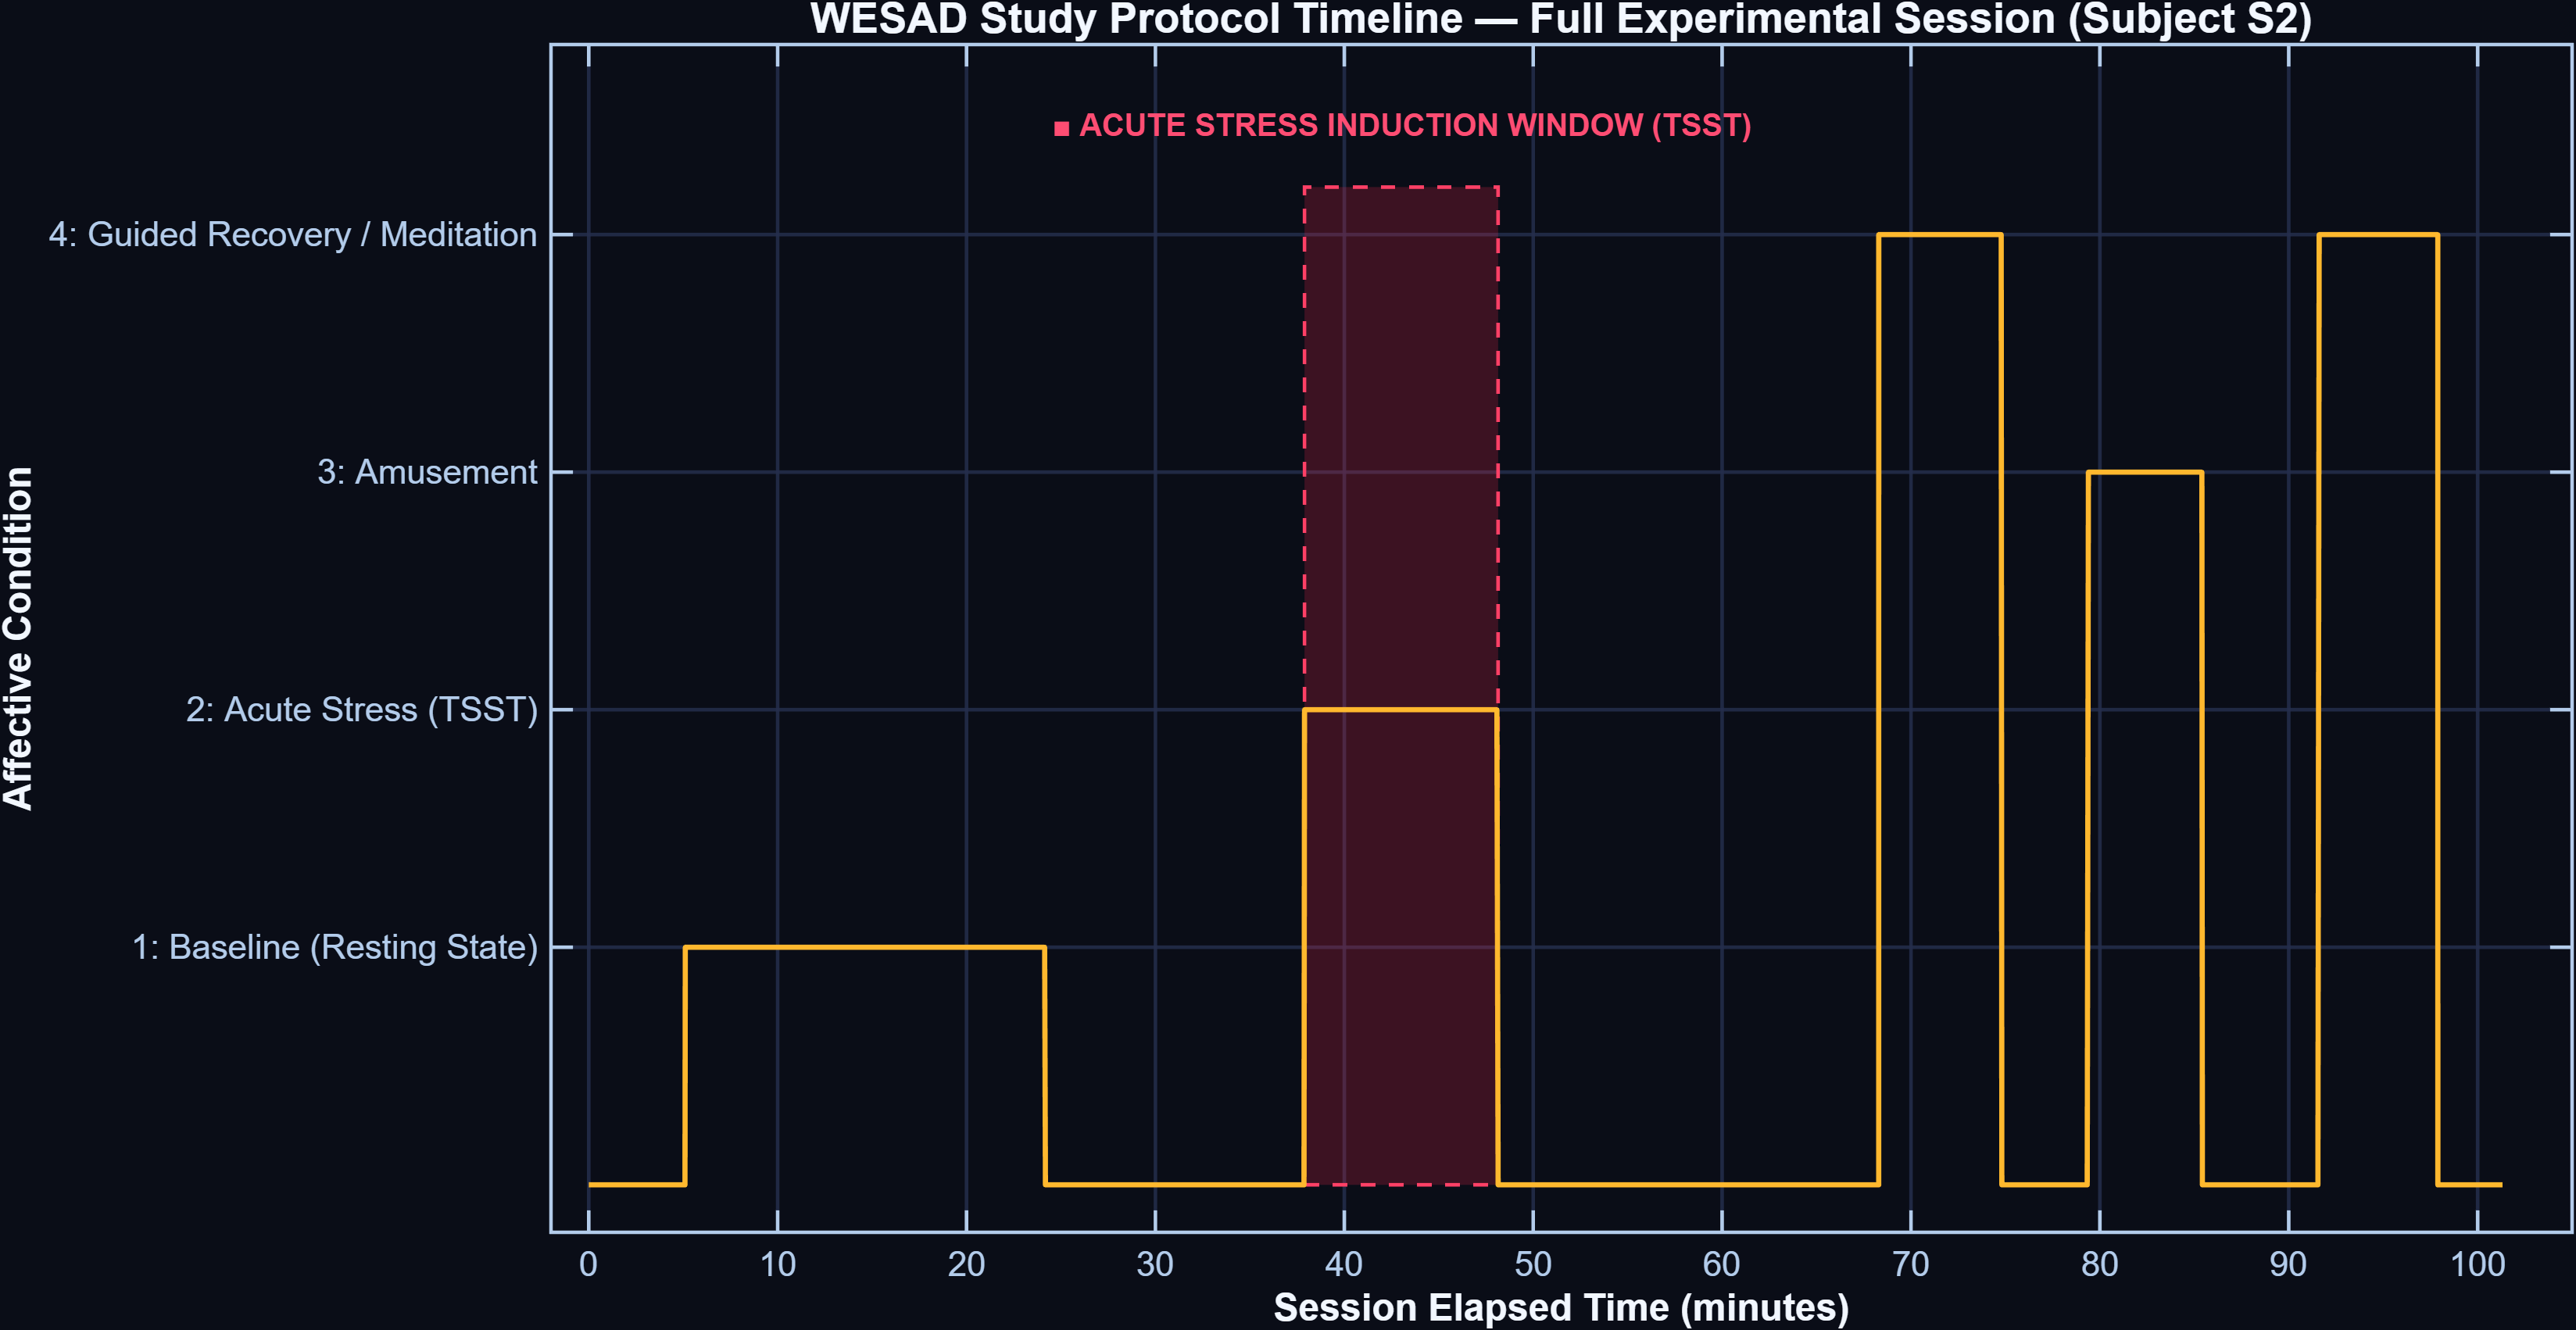
\includegraphics[width=\columnwidth]{figures/DEMO_Protocol_Timeline.png}
    \caption{Experimental timeline and laboratory protocol for the WESAD study~\cite{schmidt2018wesad}. The protocol progresses through an initial baseline period (seated neutral reading, 20\,min), Trier Social Stress Test (TSST: public speaking and mental arithmetic, 10--12\,min), relaxation/meditation (7\,min), and emotional amusement (watching comedy clips, 6\,min). In our study, 445 standardized 60\,s non-overlapping windows (285 baseline, 160 stress) are extracted across 15 subjects.}
    \label{fig:protocol_timeline}
\end{figure}

The system comprises three physical tiers:
\begin{enumerate}
    \item \textbf{Wearable Edge Node (STM32G474RE):} Captures raw Lead-II ECG at 700\,Hz (decimated or paced at 350\,Hz nominal), executes 5-stage biquad IIR digital filtering, encrypts the 20-byte telemetry frame using a 4D hyperchaotic stream cipher, appends a CRC-16-CCITT checksum, and transmits packets over UART.
    \item \textbf{Telemetry Gateway / Transport Layer:} Receives raw asynchronous byte streams at 115,200 baud, unpacks framed packets, validates CRC-16 checksums, and monitors sequence continuity and pacing timing.
    \item \textbf{Host-Side Analytics \& Dashboard:} Decrypts telemetry payloads using synchronized hyperchaotic state evolution, executes adaptive R-peak detection, extracts time-domain HRV metrics over 60\,s sliding windows, computes subject-specific relative baseline calibration ($\Delta x$), and executes trained LOSO classifiers to generate real-time acute stress probabilities.
\end{enumerate}

% -----------------------------------------------------------------------------
% Section V: Dataset and Experimental Protocol
% -----------------------------------------------------------------------------
\section{Dataset and Experimental Protocol}
\label{sec:dataset}

\subsection{The WESAD Dataset Cohort}
We utilize the public WESAD benchmark dataset collected by Schmidt \textit{et al.}~\cite{schmidt2018wesad}. The cohort comprises 15 healthy adult volunteers (labeled S2--S11, S13--S17; subjects S1 and S12 were excluded during original data acquisition due to sensor hardware malfunction). The participant group consists of 12 males and 3 females, aged $27.5 \pm 2.4$ years. Physiological signals were recorded using a chest-worn RespiBAN Professional device capturing single-lead Lead-II ECG at 700\,Hz.

\subsection{Experimental Conditions and Windowing}
The experimental protocol induces acute psychological and cognitive stress via the validated Trier Social Stress Test (TSST)~\cite{kirschbaum1993trier}, consisting of a 5-minute public speaking presentation followed by a 5-minute mental arithmetic task (rapid serial subtraction of 13 or 17 from a large prime number) under social evaluation. 

To ensure clinical relevance and eliminate temporal autocorrelation, the continuous ECG recordings are partitioned into complete, non-overlapping 60\,s windows:
\begin{equation}
    W_k = [k \cdot T_{\text{hop}},\, k \cdot T_{\text{hop}} + T_{\text{win}}], \quad T_{\text{win}} = 60\,\text{s},\, T_{\text{hop}} = 60\,\text{s}
    \label{eq:windowing}
\end{equation}
A 60\,s window hop step with a 60\,s window duration enforces \textbf{0\% window overlap}. Across all 15 subjects, this partitioning yields exactly \textbf{445 complete windows}:
\begin{itemize}
    \item \textbf{Baseline / Calm Windows ($y = 0$):} 285 windows (64.04\% of cohort), recorded during seated neutral reading ($\approx 19$ windows per participant).
    \item \textbf{Acute Stress Windows ($y = 1$):} 160 windows (35.96\% of cohort), recorded during the public speaking and mental arithmetic tasks (10--12 windows per participant).
\end{itemize}

Every window contains exactly 42,000 raw ECG samples at 700\,Hz. All 445 windows contain zero missing values (NaN) and zero duplicated rows, verified cryptographically via SHA-256 hash \texttt{0405170b...} in \texttt{WESAD\_HRV\_features\_expanded.csv}.

% -----------------------------------------------------------------------------
% Section VI: ECG Preprocessing and HRV Feature Extraction
% -----------------------------------------------------------------------------
\section{ECG Preprocessing and HRV Feature Extraction}
\label{sec:preprocessing}

\subsection{Digital Filtering and R-Peak Detection}
Raw ECG signals suffer from respiration-induced baseline wander ($<0.5$\,Hz), powerline electromagnetic interference (50/60\,Hz), and high-frequency electromyographic (EMG) muscle noise ($>40$\,Hz). 

\begin{figure}[t]
    \centering
    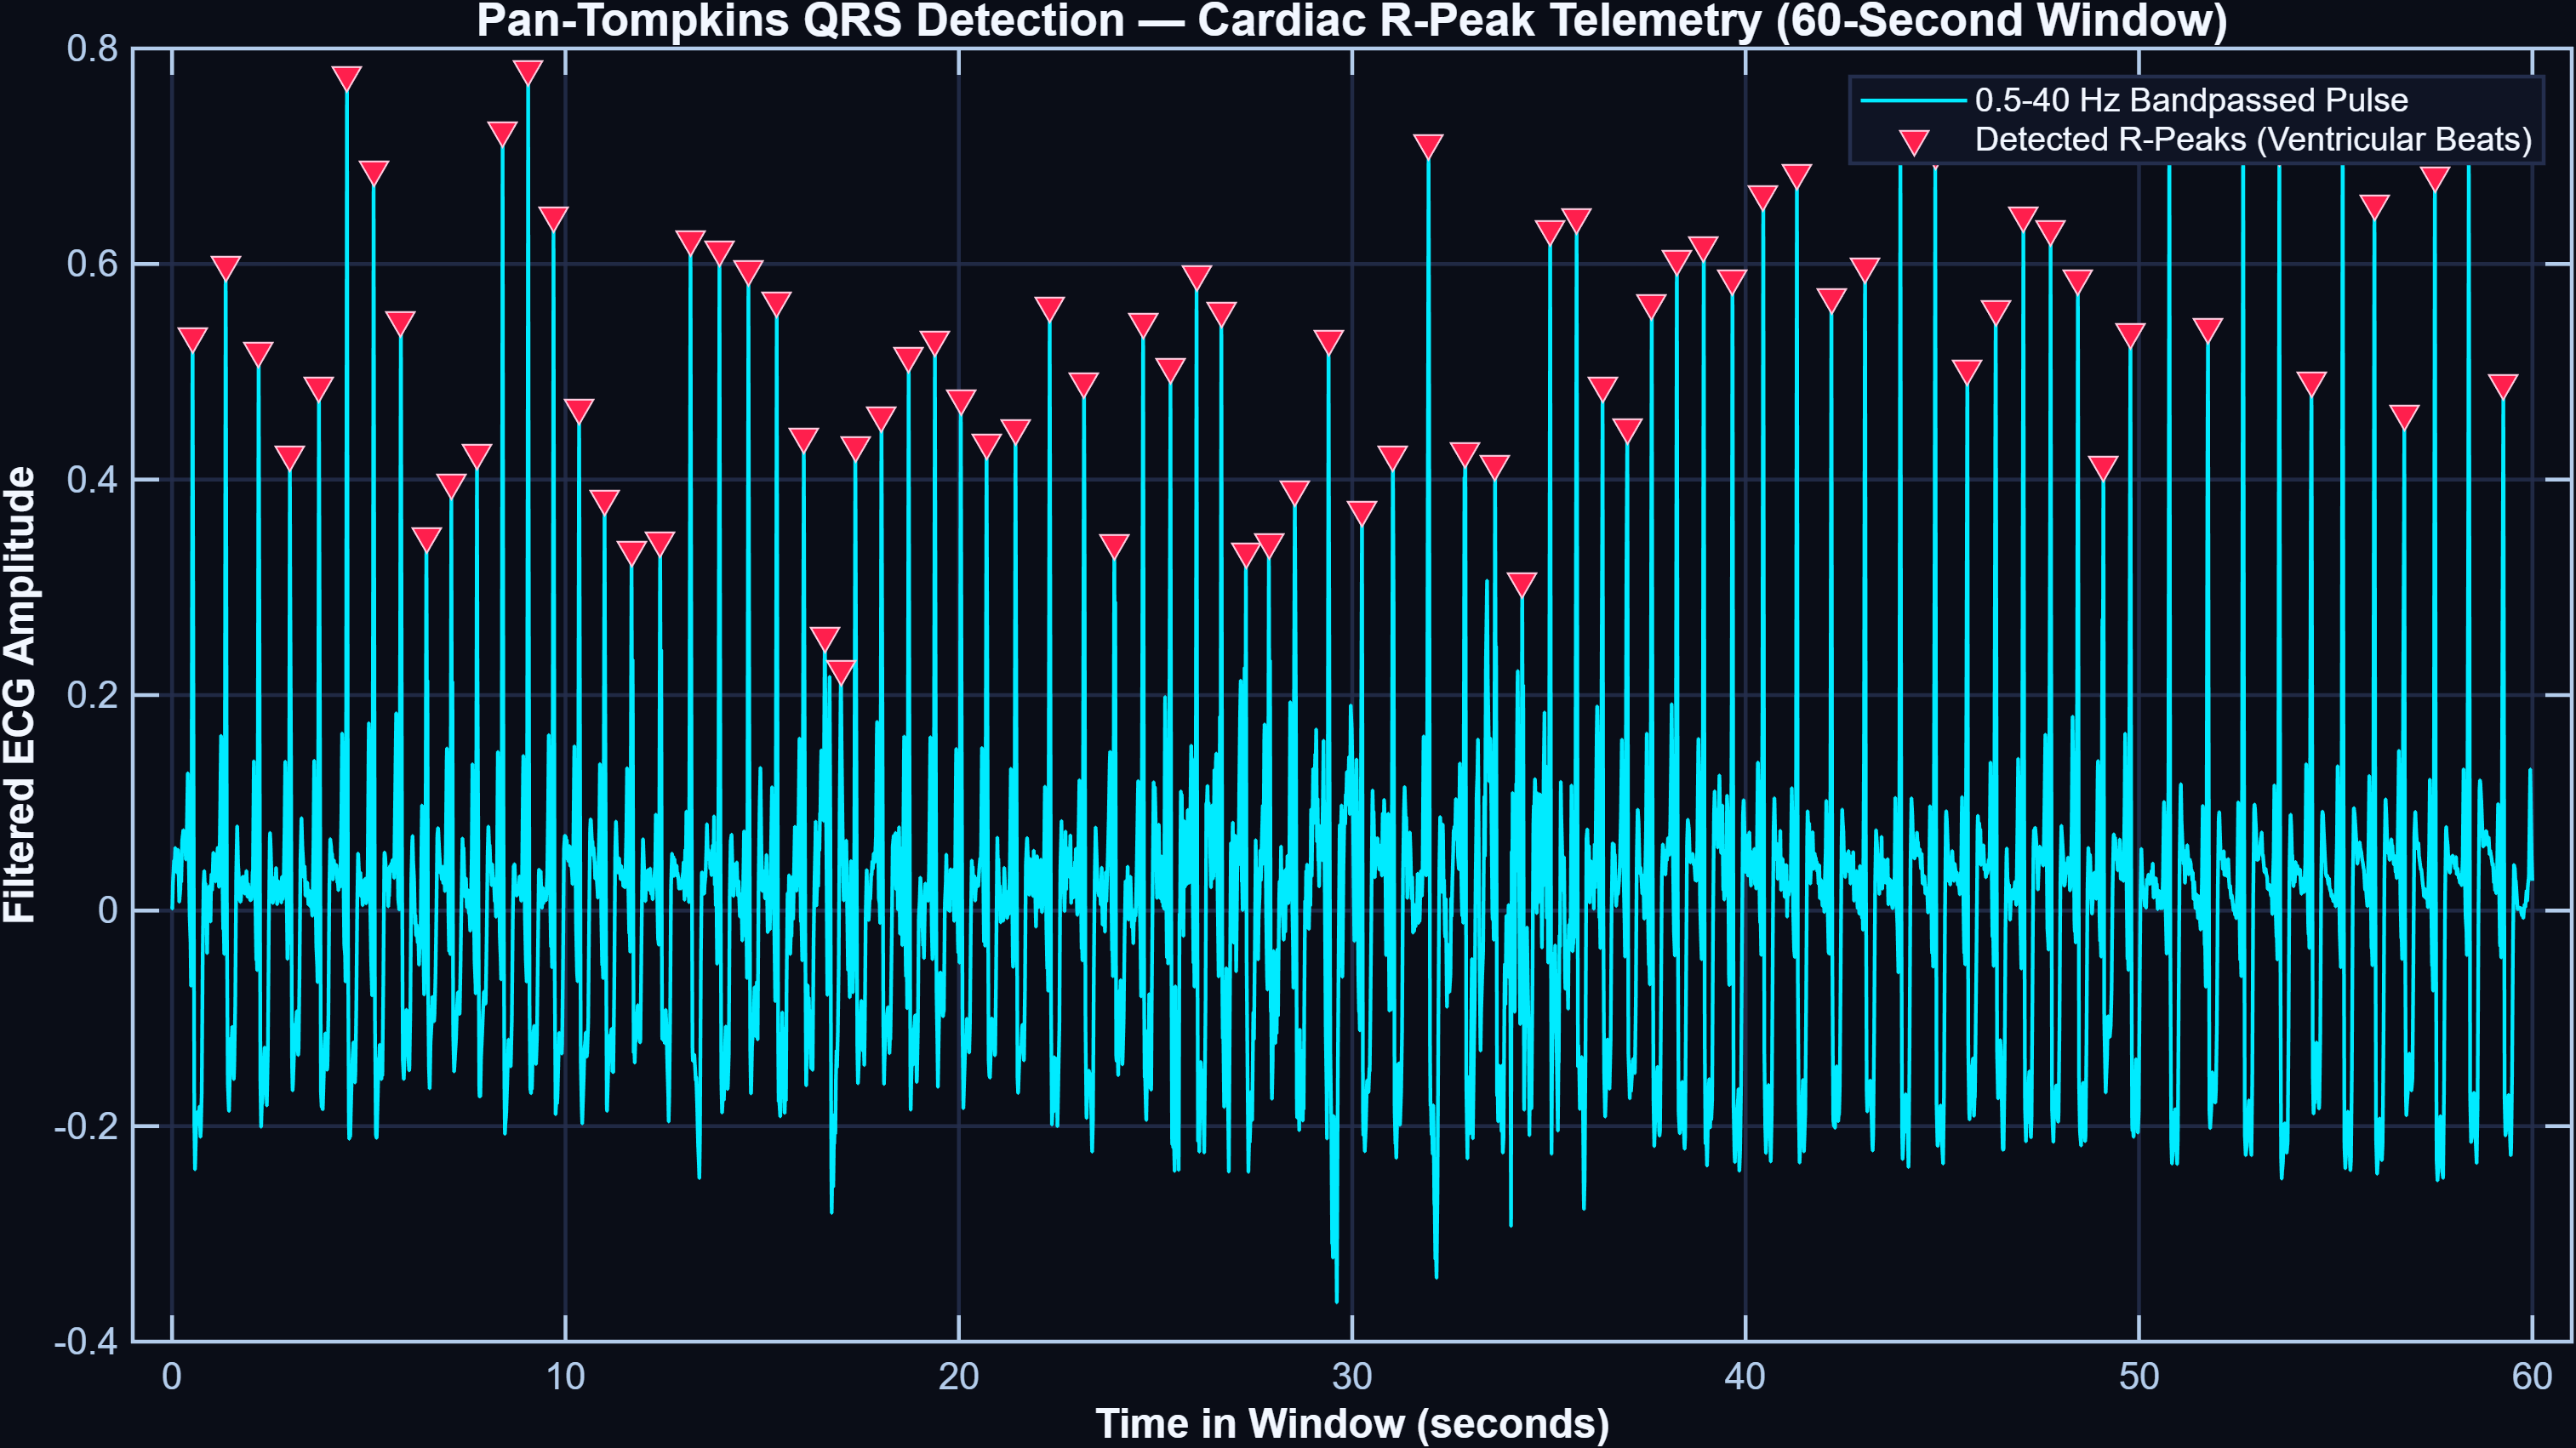
\includegraphics[width=\columnwidth]{figures/DEMO_Pan_Tompkins_QRS_Detection.png}
    \caption{ECG preprocessing and Pan-Tompkins QRS detection pipeline. (a)~Raw Lead-II ECG showing baseline wander and high-frequency noise. (b)~Filtered ECG after 4th-order Butterworth bandpass (0.5--40\,Hz). (c)~First-difference derivative signal highlighting steep QRS slopes. (d)~Squared derivative amplifying R-peaks while suppressing P and T waves. (e)~Moving-window integrator with adaptive threshold detecting R-peak events.}
    \label{fig:pan_tompkins}
\end{figure}

The offline preprocessing pipeline in MATLAB applies a zero-phase 4th-order Butterworth bandpass filter:
\begin{equation}
    H(s) = \frac{(\frac{s}{\omega_L})^2}{\left(s^2 + \frac{\omega_L}{Q}s + \omega_L^2\right)\left(s^2 + \frac{\omega_H}{Q}s + \omega_H^2\right)}
    \label{eq:butterworth}
\end{equation}
with cutoff frequencies $f_L = 0.5$\,Hz and $f_H = 40.0$\,Hz implemented via bidirectional filtering (\texttt{filtfilt}) to eliminate phase distortion. 

For robust R-peak detection across diverse morphologies, we employ an adaptive Median Absolute Deviation (MAD) noise-floor estimator (Fig.~\ref{fig:pan_tompkins}):
\begin{equation}
    \sigma_{\text{MAD}} = 1.4826 \cdot \text{median}\left(\left| x[n] - \text{median}(x[n]) \right|\right)
    \label{eq:mad}
\end{equation}
Candidate peaks are detected by enforcing an adaptive prominence constraint:
\begin{equation}
    \text{Prominence}(p) \ge 3.0 \cdot \sigma_{\text{MAD}}
    \label{eq:prominence}
\end{equation}
followed by a biological refractory blanking interval of $\Delta t_{\text{ref}} = 350$\,ms, bounding maximum allowable instantaneous heart rate to 171\,BPM. 

Normal-to-normal RR intervals are computed as:
\begin{equation}
    RR_i = t_{R, i+1} - t_{R, i}
    \label{eq:rr_interval}
\end{equation}
and gated through physiological plausibility boundaries:
\begin{equation}
    0.30\,\text{s} \le RR_i \le 1.50\,\text{s} \quad (40\,\text{BPM} \le \text{HR}_i \le 200\,\text{BPM})
    \label{eq:rr_gating}
\end{equation}
Any interval outside this envelope is rejected as an ectopic beat or motion artifact. Windows containing fewer than 5 valid detected beats are discarded.

\subsection{HRV Feature Extraction}
From the validated normal RR series in each 60\,s window, 13 time-domain and statistical metrics are computed. For the primary deployable model, an 8-feature representation is selected:
\begin{equation}
\begin{aligned}
    \mathbf{X} = [ & \text{MeanHR},\, \text{SDNN},\, \text{RMSSD},\, \text{pNN50}, \\
                   & \text{MeanRR},\, \text{RR}_{\text{CV}},\, \text{RR}_{\text{IQR}},\, \text{HR}_{\text{IQR}}]
\end{aligned}
\label{eq:feature_vector}
\end{equation}
Mathematical formulations for these core metrics are defined as follows:

\begin{enumerate}
    \item \textbf{Mean Heart Rate ($\text{MeanHR}$):} Average beats per minute:
    \begin{equation}
        \text{MeanHR} = \frac{60}{N} \sum_{i=1}^{N} \frac{1}{RR_i} \quad [\text{BPM}]
    \end{equation}
    \item \textbf{Standard Deviation of NN Intervals ($\text{SDNN}$):} Total autonomic variability:
    \begin{equation}
        \text{SDNN} = \sqrt{\frac{1}{N-1} \sum_{i=1}^{N} (RR_i - \overline{RR})^2} \quad [\text{s}]
    \end{equation}
    \item \textbf{Root Mean Square of Successive Differences ($\text{RMSSD}$):} Primary marker of parasympathetic vagal modulation:
    \begin{equation}
        \text{RMSSD} = \sqrt{\frac{1}{N-1} \sum_{i=1}^{N-1} (RR_{i+1} - RR_i)^2} \quad [\text{s}]
    \end{equation}
    \item \textbf{Percentage of Successive Differences $> 50$\,ms ($\text{pNN50}$):} High-frequency parasympathetic tone:
    \begin{equation}
        \text{pNN50} = \frac{1}{N-1} \sum_{i=1}^{N-1} \mathbb{I}(|RR_{i+1} - RR_i| > 0.05\,\text{s}) \times 100\%
    \end{equation}
    \item \textbf{Coefficient of Variation ($\text{RR}_{\text{CV}}$):} Normalized variability:
    \begin{equation}
        \text{RR}_{\text{CV}} = \frac{\text{SDNN}}{\overline{RR}} \quad [\text{dimensionless ratio}]
    \end{equation}
    \item \textbf{Interquartile Ranges ($\text{RR}_{\text{IQR}}$, $\text{HR}_{\text{IQR}}$):} Non-parametric dispersion robust against transient ectopic outliers:
    \begin{equation}
        \text{IQR}(z) = Q_3(z) - Q_1(z)
    \end{equation}
\end{enumerate}

% -----------------------------------------------------------------------------
% Section VII: Machine-Learning Methodology
% -----------------------------------------------------------------------------
\section{Machine-Learning Methodology}
\label{sec:ml_methodology}

\subsection{Subject-Specific Relative Baseline Normalization ($\Delta x$)}
The core methodological breakthrough of our framework is the subject-specific relative baseline calibration. For any physiological metric $x$ in window $j$ of subject $s$, we define the relative fractional displacement $\Delta x_{s,j}$ with respect to that individual's calm baseline centroid $\mu_{\text{base}, s}$:
\begin{equation}
    \Delta x_{s,j} = \frac{x_{s,j} - \mu_{\text{base}, s}}{\max\left(|\mu_{\text{base}, s}|,\, 10^{-6}\right)}
    \label{eq:baseline_calibration}
\end{equation}
where $\mu_{\text{base}, s} = \frac{1}{M_s} \sum_{m=1}^{M_s} x_{s, m}^{\text{calm}}$ is computed strictly across the $M_s$ resting baseline windows of subject $s$. 

\begin{figure}[t]
    \centering
    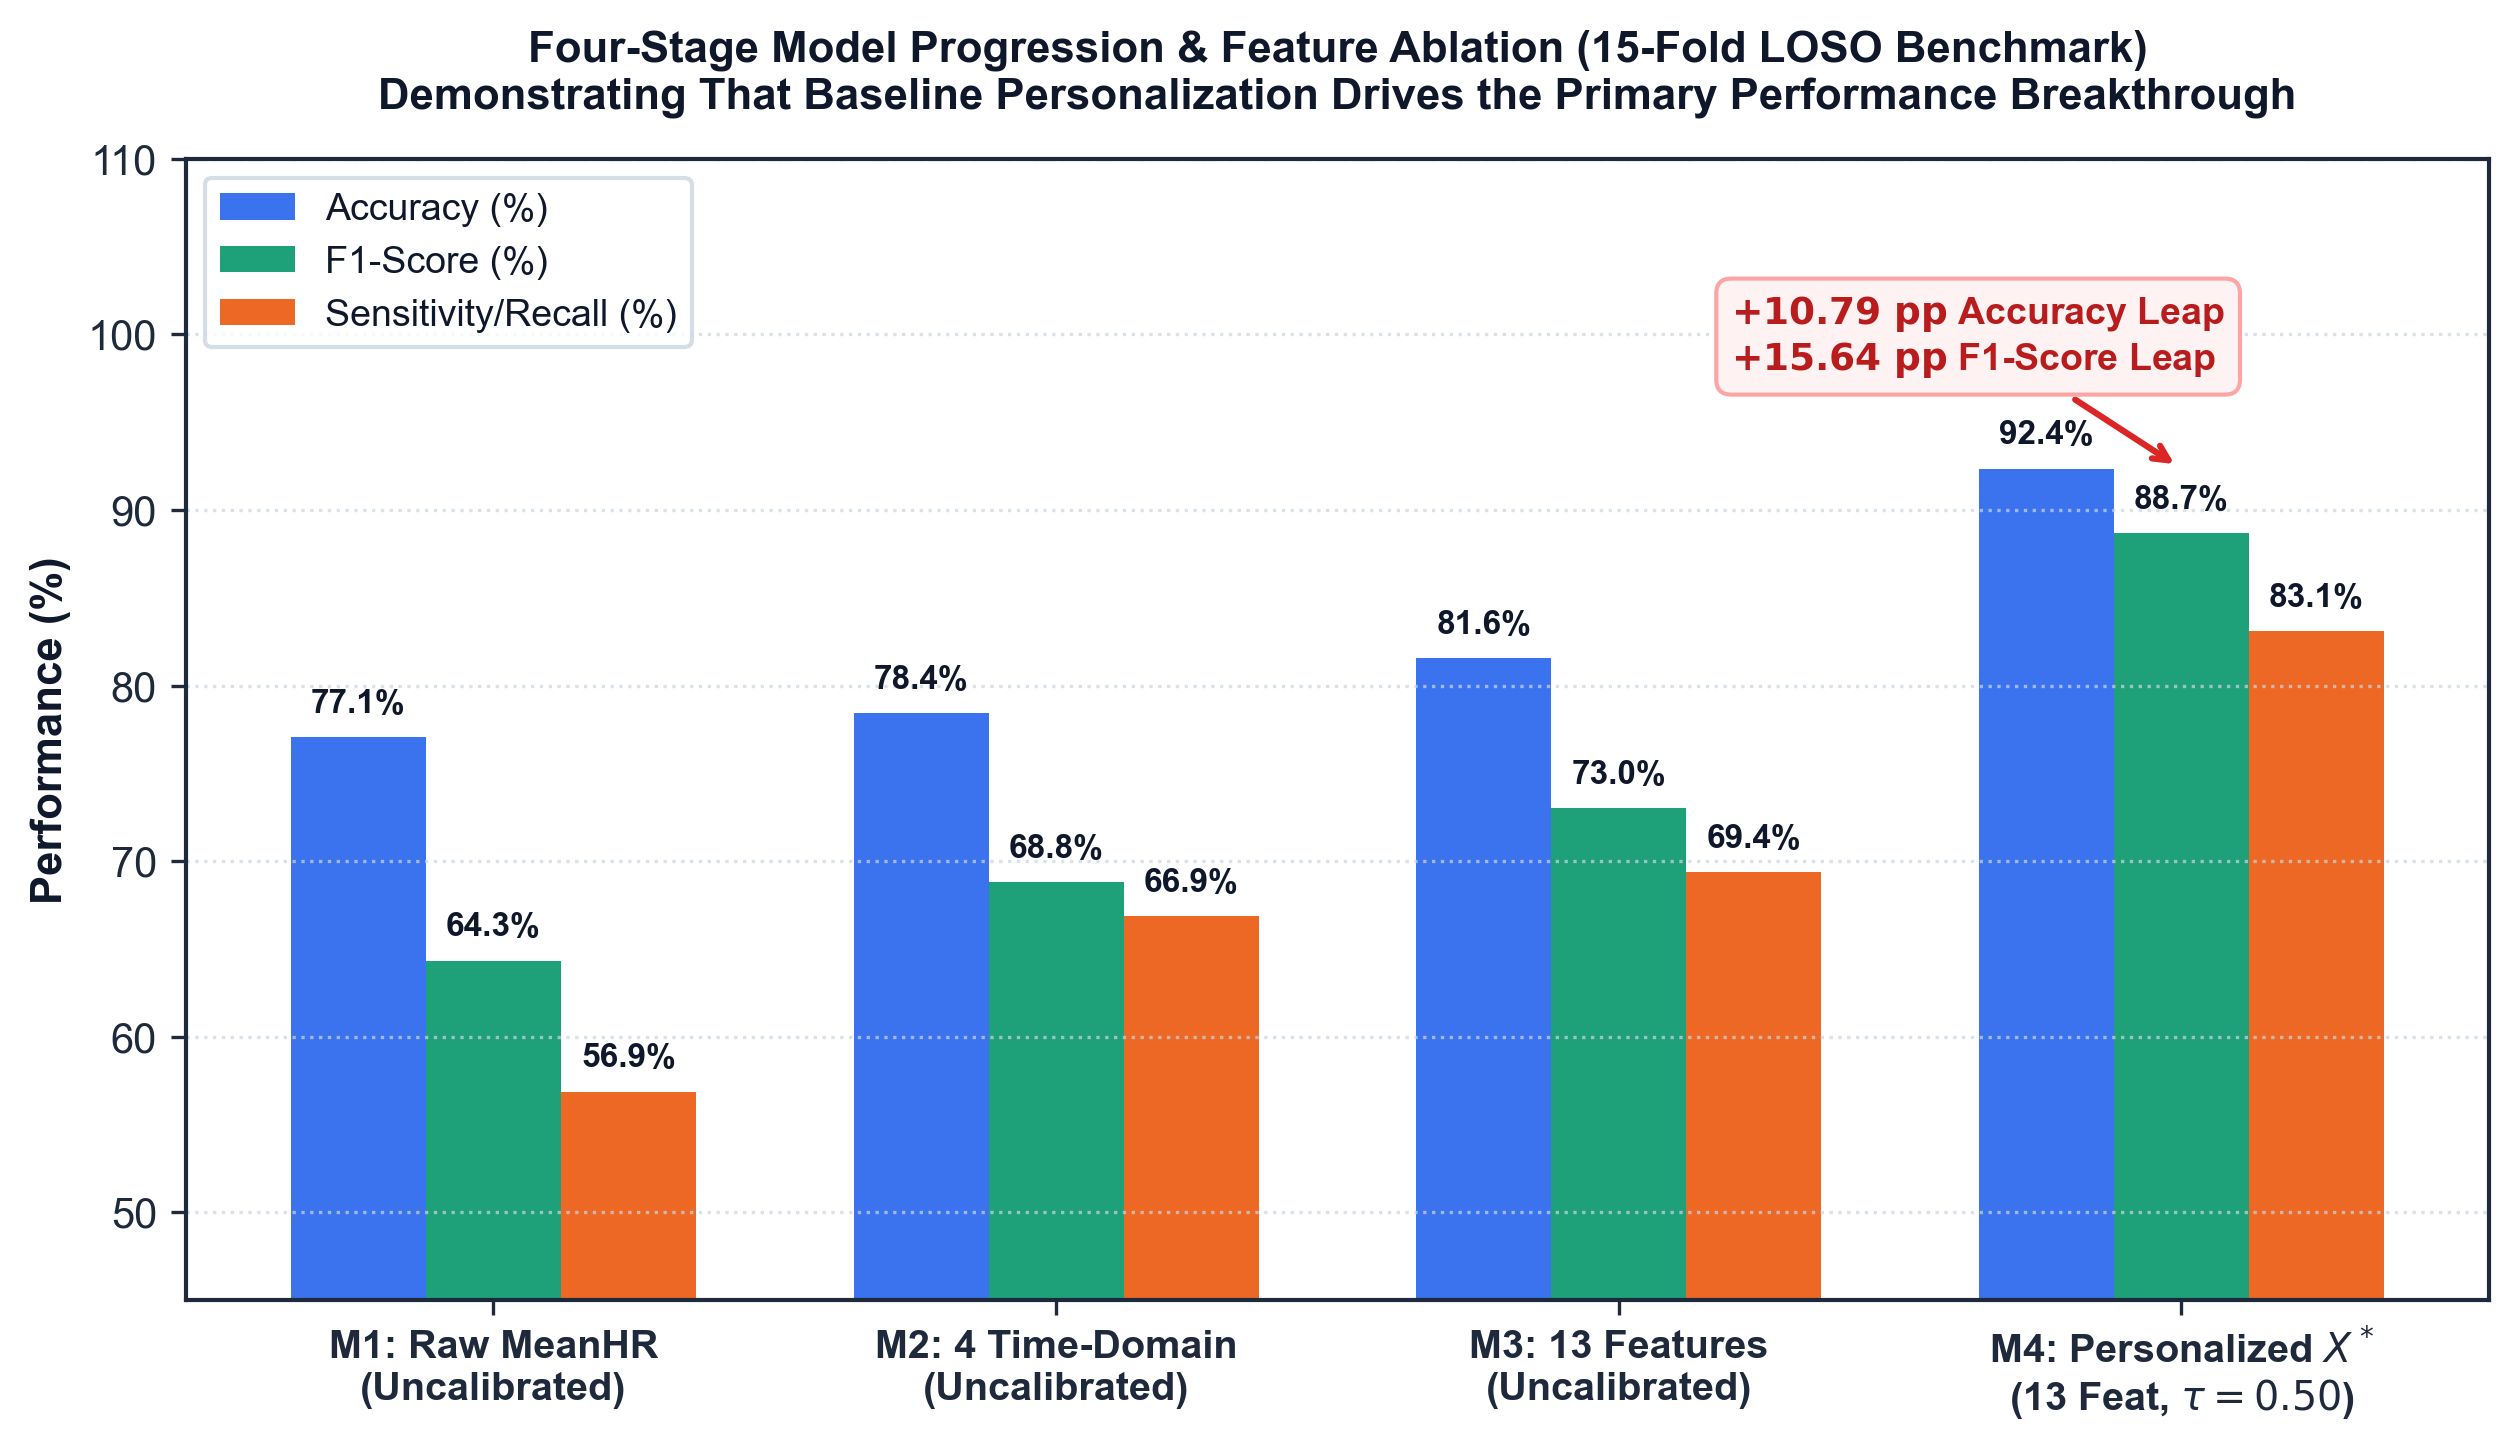
\includegraphics[width=\columnwidth]{figures/FINAL_Personalized_Feature_Ablation.png}
    \caption{Personalized feature ablation progression across four model tiers (M1--M4) at $\tau = 0.50$. M1 (Raw MeanHR, uncalibrated) yields 77.08\% accuracy. M2 (4 time-domain features) yields 78.43\%. M3 (13 raw features) yields 81.57\%. M4 (Personalized baseline calibration $\Delta x$ across 13 features) reaches 92.36\% accuracy and 88.67\% F1-score, delivering a $+10.79$ percentage-point leap over uncalibrated metrics.}
    \label{fig:ablation_study}
\end{figure}

This transformation possesses two critical properties:
\begin{enumerate}
    \item It converts absolute physiological values (e.g., an individual resting at 55\,BPM vs. 85\,BPM) into dimensionless relative autonomic shifts ($\Delta\text{MeanHR} > 0$, $\Delta\text{RMSSD} < 0$), rendering feature spaces comparable across diverse subjects.
    \item In practical deployment, a 2-to-5 minute resting calibration during device setup establishes $\mu_{\text{base}}$, allowing all subsequent streaming windows to be normalized immediately.
\end{enumerate}

\subsection{Zero-Leakage 15-Fold Leave-One-Subject-Out (LOSO) Protocol}
To evaluate real-world cross-subject generalization, we enforce a strict 15-fold LOSO cross-validation scheme:
\begin{itemize}
    \item In fold $k \in \{1, \dots, 15\}$, subject $k$ is held out as the test set ($D_{\text{test}}^{(k)}$).
    \item The classifier is trained strictly on the remaining 14 subjects ($D_{\text{train}}^{(k)}$).
    \item A standard z-score scaler (\texttt{StandardScaler}) is fitted \textbf{strictly} on $D_{\text{train}}^{(k)}$:
    \begin{equation}
        z = \frac{\Delta x - \mu_{\text{train}}}{\sigma_{\text{train}}}
        \label{eq:zscore}
    \end{equation}
    and applied to transform both $D_{\text{train}}^{(k)}$ and $D_{\text{test}}^{(k)}$.
    \item For test subject $k$, baseline centroid $\mu_{\text{base}}^{(k)}$ is computed strictly from subject $k$'s own baseline windows ($y=0$); test stress windows and test labels are never exposed during training or scaling.
\end{itemize}

\subsection{Classifier Architectures and Hyperparameters}
We benchmark six distinct supervised learning architectures:
\begin{enumerate}
    \item \textbf{Logistic Regression (Primary Model):} L2-regularized linear model with coordinate descent solver (\texttt{liblinear}), inverse regularization strength $C = 1.0$, and tolerance $\epsilon = 10^{-4}$. Minimizes the objective:
    \begin{equation}
        \min_{\mathbf{w}, b} \frac{1}{2} \|\mathbf{w}\|_2^2 + C \sum_{i=1}^{M} \log\left(1 + e^{-y_i (\mathbf{w}^T \mathbf{z}_i + b)}\right)
        \label{eq:logreg_loss}
    \end{equation}
    \item \textbf{Support Vector Machine (SVM):} Radial Basis Function (RBF) kernel, $C = 1.5$, $\gamma = \text{scale}$, with Platt scaling for probability calibration.
    \item \textbf{Random Forest:} Ensemble of 100 decision trees, maximum depth $d = 6$, minimum split samples $s_{\min} = 4$.
    \item \textbf{Extra Trees:} Extremely randomized trees, 100 estimators, $d = 6$, $s_{\min} = 4$.
    \item \textbf{HistGradientBoosting:} Histogram-based gradient boosting, 100 boosting iterations, maximum depth $d = 4$, learning rate $\eta = 0.08$.
    \item \textbf{Multi-Layer Perceptron (MLP):} Feedforward neural network with two hidden layers $(32, 16)$, ReLU activations, Adam optimizer, initial learning rate $\alpha = 0.005$, L2 penalty $\alpha = 0.01$, and maximum 1000 iterations.
\end{enumerate}

All classifiers are initialized with \texttt{random\_state = 42} to guarantee exact mathematical reproducibility.

\subsection{Dual-Threshold Decision Framework}
Predicted probabilities $P(\text{Stress} \mid \mathbf{z}) = \sigma(\mathbf{w}^T \mathbf{z} + b)$ are evaluated across two operational thresholds:
\begin{itemize}
    \item \textbf{Primary Scientific Benchmark ($\tau = 0.50$):} Unbiased theoretical decision boundary:
    \begin{equation}
        \hat{y} = \mathbb{I}(P(\text{Stress} \mid \mathbf{z}) \ge 0.50)
    \end{equation}
    Prioritizes high specificity (97.54\%) to minimize disruptive false positive alarms in daily ambulatory monitoring.
    \item \textbf{Exploratory Clinical-Screening Point ($\tau = 0.35$):} Sensitivity-prioritized operating point:
    \begin{equation}
        \hat{y} = \mathbb{I}(P(\text{Stress} \mid \mathbf{z}) \ge 0.35)
    \end{equation}
    Prioritizes stress detection recall (capturing 86.25\% of acute stress episodes) for clinical triage.
\end{itemize}

% -----------------------------------------------------------------------------
% Section VIII: Embedded STM32 Telemetry System
% -----------------------------------------------------------------------------
\section{Embedded STM32 Telemetry System}
\label{sec:embedded_system}

\subsection{Microcontroller Hardware Platform}
The embedded edge prototype is implemented on the STMicroelectronics NUCLEO-G474RE development board, featuring an ARM Cortex-M4 32-bit RISC core operating at 170\,MHz SYSCLK, an integrated single-precision Floating Point Unit (FPU), 512\,kB Flash memory, and 128\,kB SRAM~\cite{stmicroelectronics2020stm32g4}.

\begin{figure}[t]
    \centering
    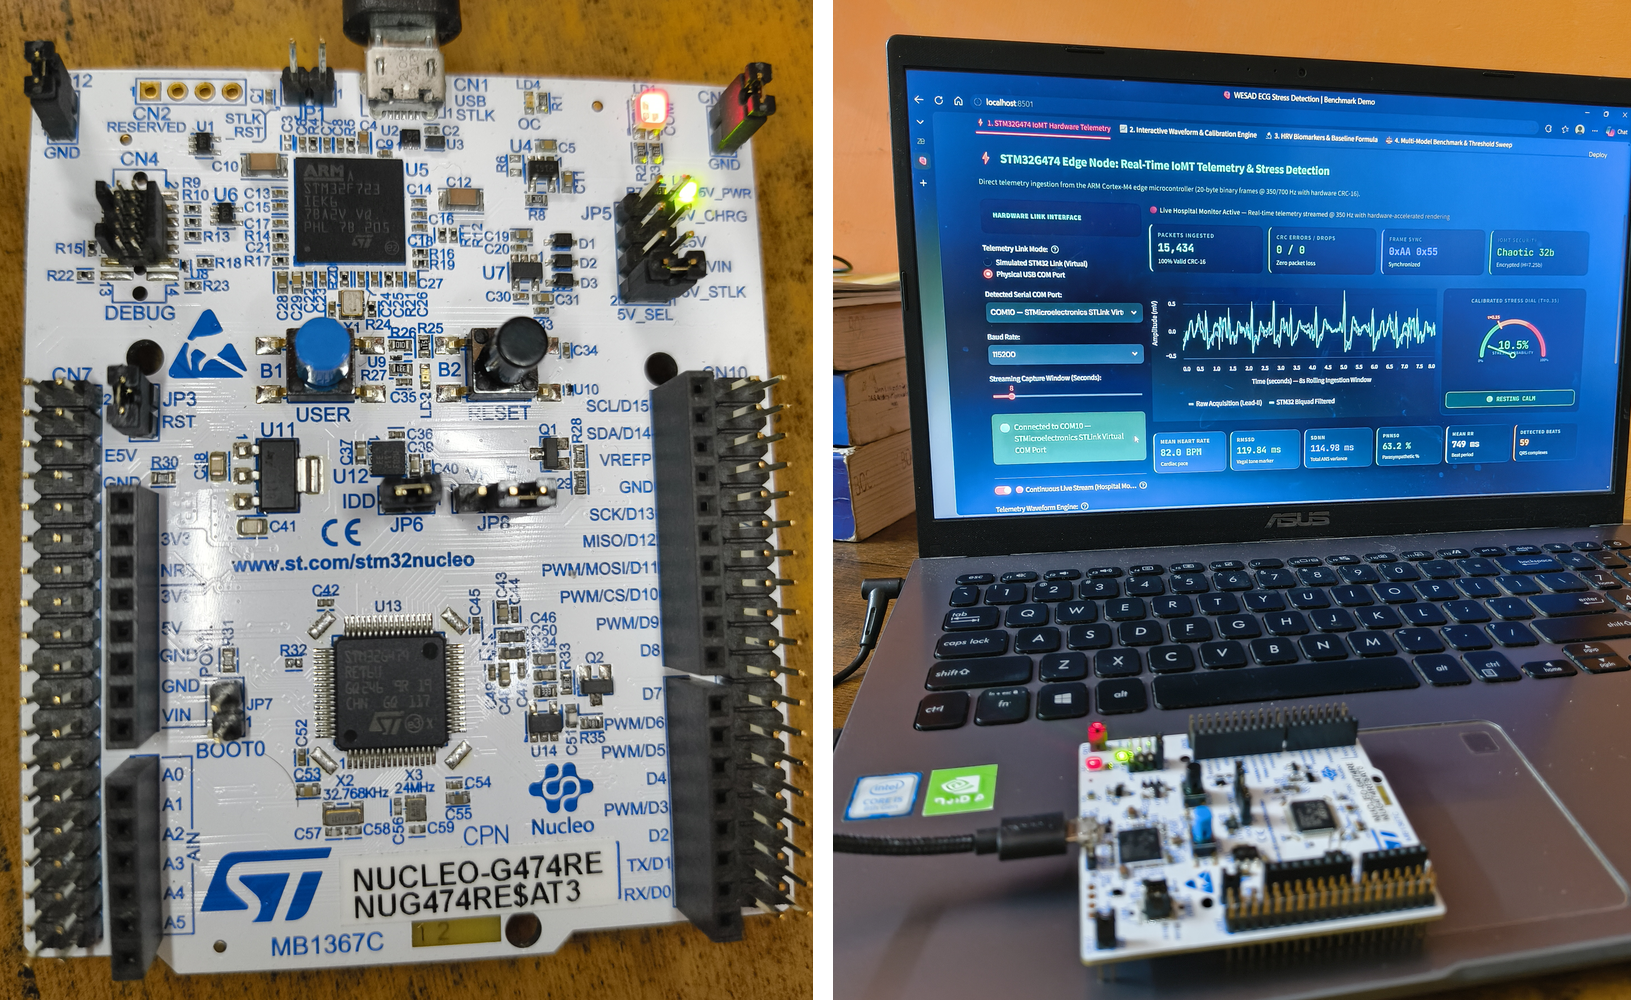
\includegraphics[width=\columnwidth]{figures/FIG_Hardware_Testbed_Composite.png}
    \caption{Laboratory hardware-in-the-loop (HIL) testbench. The STM32G474RE Nucleo-64 board executes real-time 5-stage Biquad IIR filtering and 4D hyperchaotic telemetry encryption. Streaming packets are transmitted over the ST-Link Virtual COM Port (115,200 baud) to the host reception console.}
    \label{fig:hardware_testbed}
\end{figure}

\subsection{Real-Time 5-Stage Direct Form I Biquad IIR Filter}
To execute real-time noise suppression on-device, we implement a 5-stage cascaded Direct Form~I Biquad IIR digital filter (4 stages for 4th-order Butterworth 0.5--40\,Hz bandpass plus 1 stage for 50\,Hz notch, quality factor $Q = 30$). 

Each biquad second-order section (SOS) is computed via the difference equation:
\begin{equation}
    y[n] = b_0 x[n] + b_1 x[n-1] + b_2 x[n-2] - a_1 y[n-1] - a_2 y[n-2]
    \label{eq:biquad}
\end{equation}
Implemented using ARM CMSIS-DSP single-precision floating-point functions (\texttt{arm\_biquad\_cascade\_df1\_f32})~\cite{arm2021cmsis}, execution of all 5 cascaded stages requires approximately 318 CPU cycles ($1.87\,\mu\text{s}$ at 170\,MHz SYSCLK). At the nominal 350\,Hz sampling rate ($T_s = 2.857$\,ms), digital filtering consumes only \textbf{0.065\%} of the available inter-sample CPU processing budget.

\subsection{Telemetry Packet Framing Protocol}
Telemetry data is encapsulated into fixed-size 20-byte frames (Table~\ref{tab:frame_structure}) transmitted over UART at 115,200 baud, 8 data bits, no parity, 1 stop bit (8N1):

\begin{table}[h]
\centering
\caption{20-Byte Embedded Telemetry Frame Structure}
\label{tab:frame_structure}
\footnotesize
\setlength{\tabcolsep}{2.5pt}
\begin{tabular}{@{}llcp{3.5cm}@{}}
\toprule
\textbf{Field} & \textbf{Type} & \textbf{Bytes} & \textbf{Description} \\
\midrule
\texttt{SOF} & \texttt{uint16\_t} & 2 & Synchronization header (\texttt{0xAA55}) \\
\texttt{Version} & \texttt{uint8\_t} & 1 & Protocol version (\texttt{0x01}) \\
\texttt{Flags} & \texttt{uint8\_t} & 1 & Mode flags (\texttt{0x05}: \texttt{ENCRYPTED | CHAOS}) \\
\texttt{SeqID} & \texttt{uint16\_t} & 2 & Monotonically increasing sequence ID \\
\texttt{Timestamp} & \texttt{uint32\_t} & 4 & Hardware SysTick counter (ms) \\
\texttt{RawECG} & \texttt{float32} & 4 & Pre-filter single-precision sample \\
\texttt{FiltECG} & \texttt{float32} & 4 & On-device filtered sample \\
\texttt{CRC16} & \texttt{uint16\_t} & 2 & CRC-16-CCITT checksum (\texttt{0x1021}) \\
\midrule
\multicolumn{2}{@{}l}{\textbf{Total Frame Size}} & \textbf{20} & \textbf{Bytes per Telemetry Packet} \\
\bottomrule
\end{tabular}
\end{table}

Data payload integrity is safeguarded by the CCITT-16 cyclic redundancy check polynomial:
\begin{equation}
    P(x) = x^{16} + x^{12} + x^5 + 1 \quad (\text{hex: } \texttt{0x1021})
    \label{eq:crc16}
\end{equation}

% -----------------------------------------------------------------------------
% Section IX: HC1 Experimental Telemetry Protection
% -----------------------------------------------------------------------------
\section{HC1 Experimental Telemetry Protection}
\label{sec:hc1_encryption}

\subsection{Nonlinear 4D Hyperchaotic Flow (M-4DCHS)}
To protect telemetry payloads against casual over-the-wire eavesdropping without incurring the heavy overhead of public-key infrastructure, we implement an experimental 4-dimensional coupled hyperchaotic system (M-4DCHS)~\cite{sprott1994some}:
\begin{equation}
\begin{aligned}
    \dot{x} &= a(y - x) + w \\
    \dot{y} &= c x - x z - y \\
    \dot{z} &= x y - b z \\
    \dot{w} &= -d x
\end{aligned}
\label{eq:hyperchaos}
\end{equation}
with system parameters $a = 35$, $b = 3$, $c = 28$, and $d = 5$. Numerical calculation yields two positive Lyapunov exponents ($\lambda_1 \approx +0.438$, $\lambda_2 \approx +0.254$), confirming hyperchaotic flow characterized by multi-directional phase-space expansion and broadband spectral power.

\subsection{Numerical Discretization and Keystream Generation}
The continuous system is integrated in real time using a 4th-order Runge-Kutta (RK4) numerical scheme with fixed integration step $h = 0.0025$:
\begin{equation}
    \mathbf{v}_{n+1} = \mathbf{v}_n + \frac{h}{6}\left(\mathbf{k}_1 + 2\mathbf{k}_2 + 2\mathbf{k}_3 + \mathbf{k}_4\right)
    \label{eq:rk4}
\end{equation}
State variables are mapped to pseudo-random keystream bytes $K_i$ via non-linear IEEE-754 floating-point mantissa bitwise extraction:
\begin{equation}
    K_i = \left(\left\lfloor |x_n| \cdot 10^7 \right\rfloor \oplus \left\lfloor |w_n| \cdot 10^7 \right\rfloor\right) \pmod{256}
    \label{eq:keystream}
\end{equation}

\subsection{Per-Packet Nonce Perturbation and CFB-8 Mixing}
To eliminate deterministic replay vulnerabilities, each packet's initial state vector is perturbed by a per-packet nonce vector combining the packet's 32-bit sequence ID and hardware SysTick timestamp:
\begin{equation}
    x_0' = x_0 + \left(\frac{(\text{SeqID} \oplus \text{Timestamp}) \pmod{1000}}{10000.0}\right)
    \label{eq:nonce_perturbation}
\end{equation}
Payload bytes are encrypted using Cipher Feedback (CFB-8) stream mixing:
\begin{equation}
    C_i = P_i \oplus K_i, \quad K_{i+1} = f_{\text{chaos}}(K_i \oplus C_i)
    \label{eq:cfb8}
\end{equation}

\subsection{Cryptographic Scope and Future Standards}
\begin{figure}[t]
    \centering
    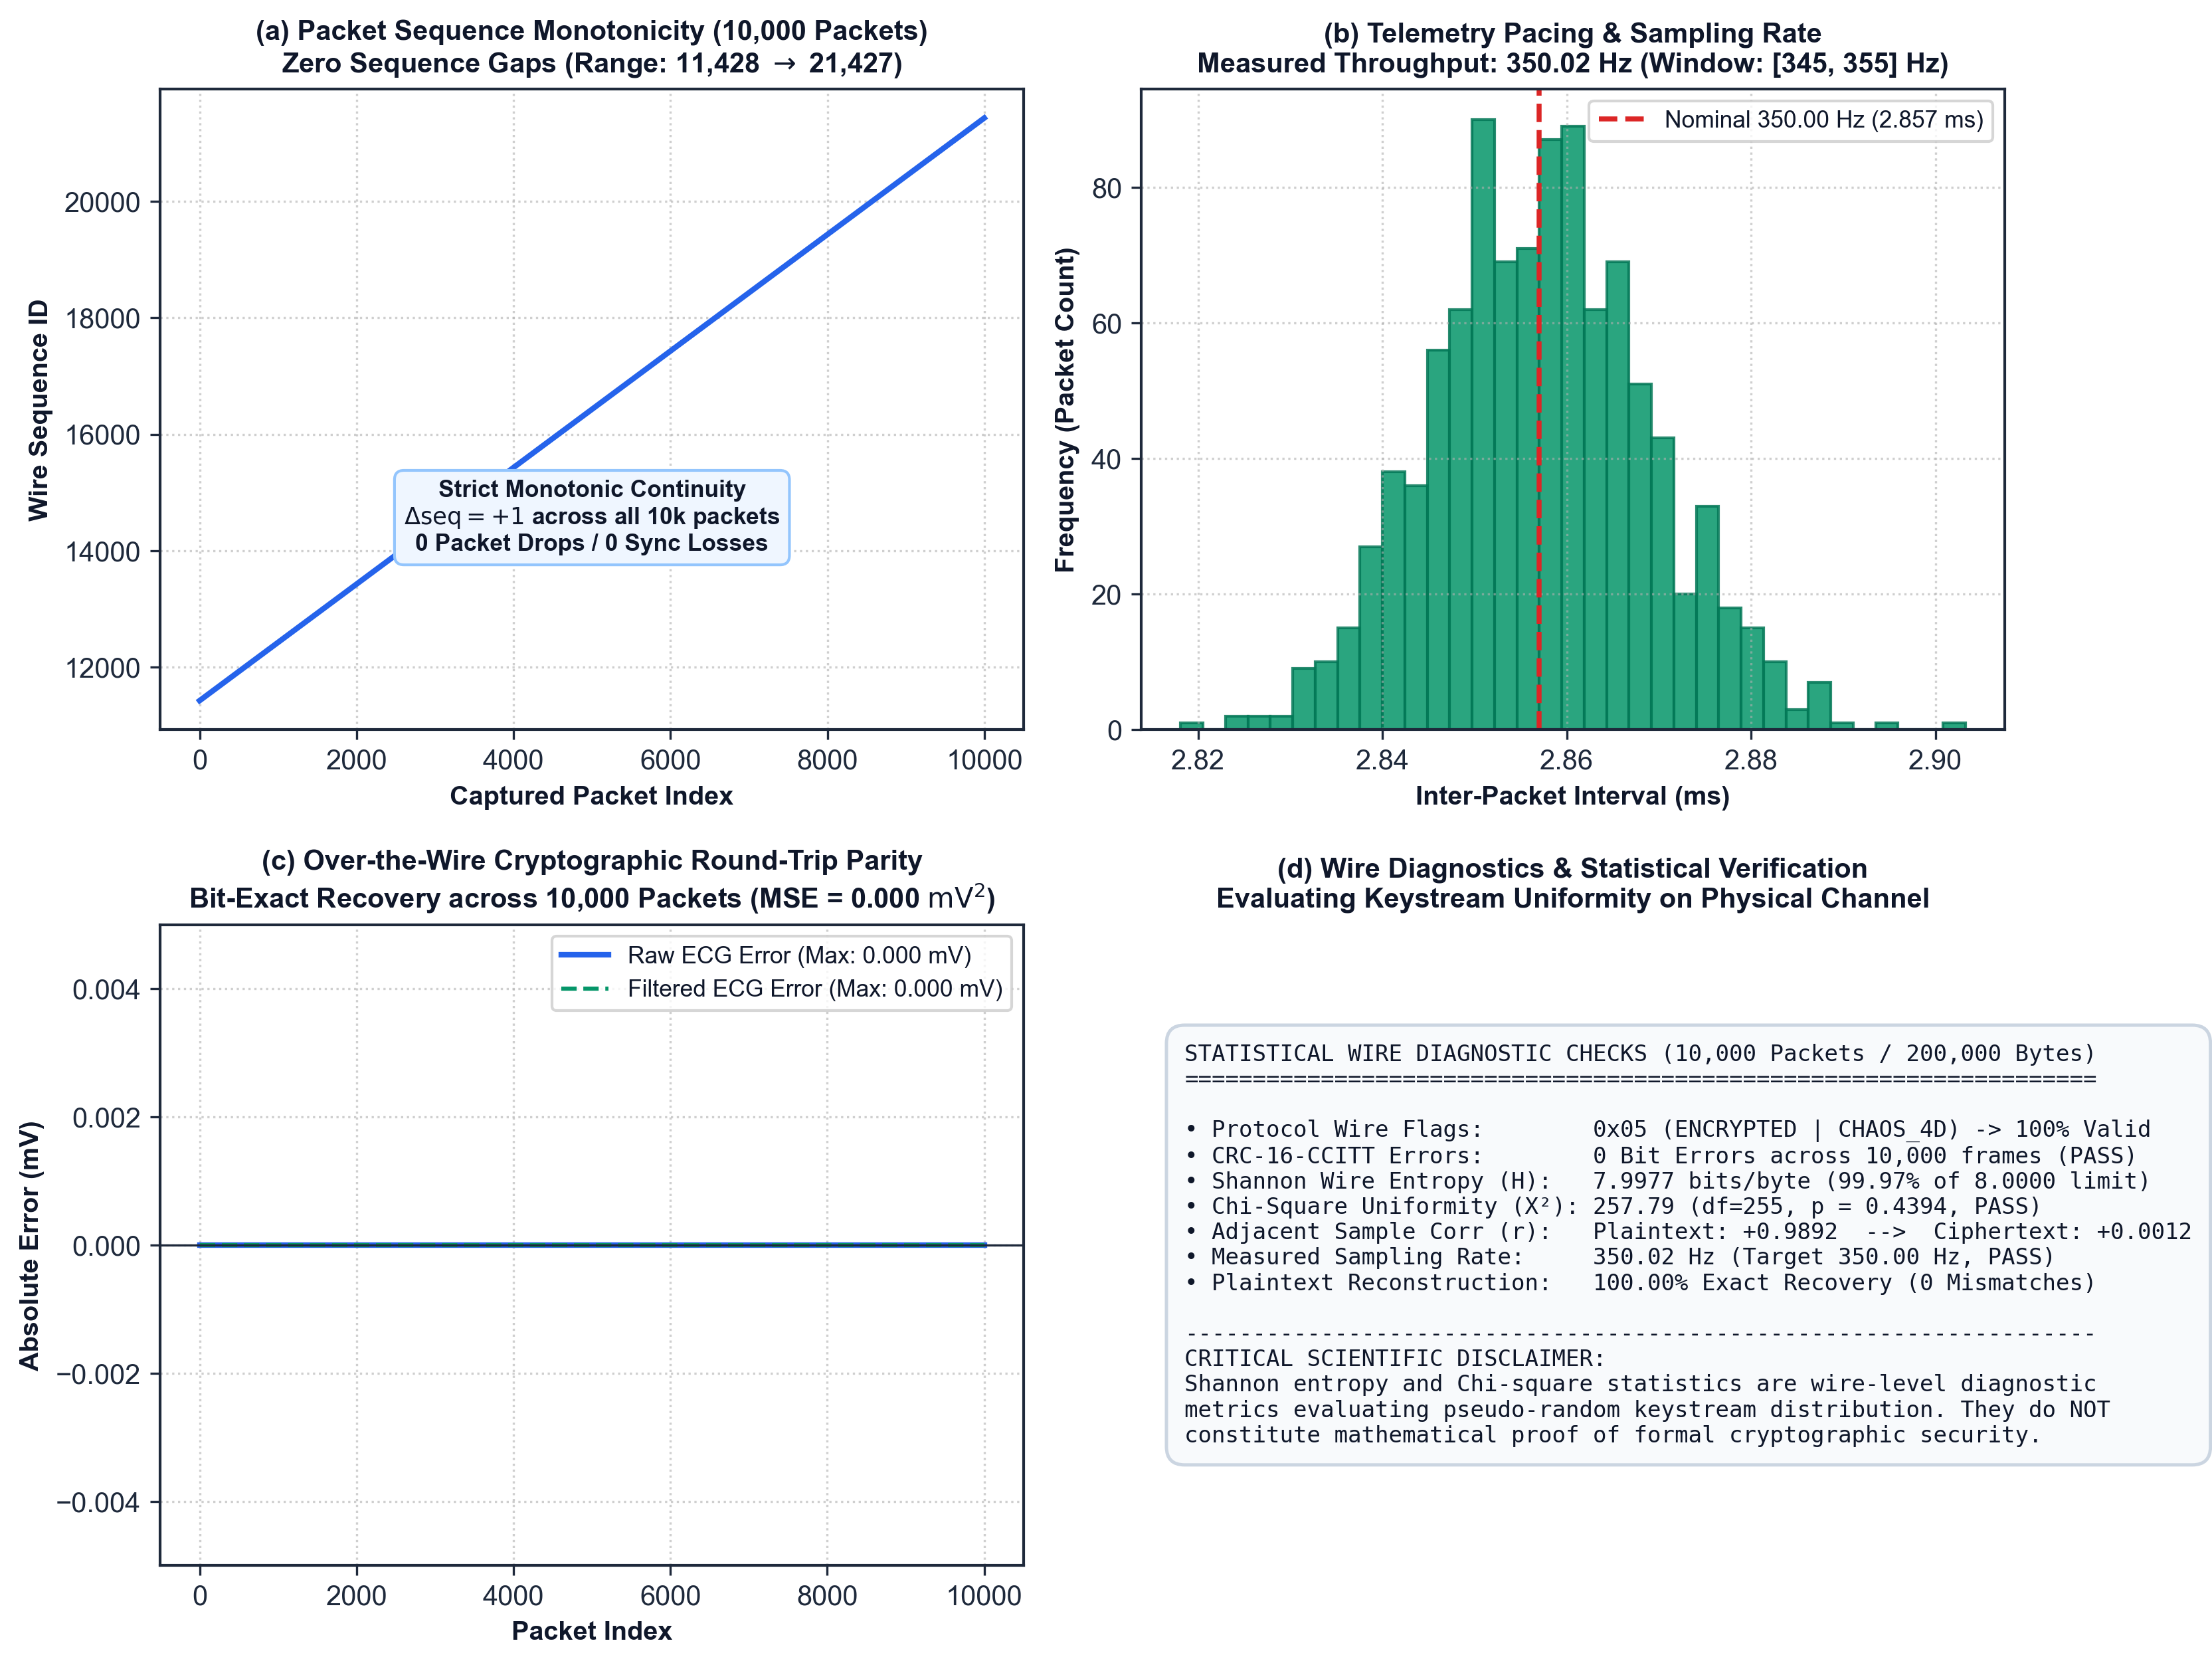
\includegraphics[width=\columnwidth]{figures/FIG_Physical_HIL_10k_Validation.png}
    \caption{Physical hardware-in-the-loop (HIL) telemetry validation across 10,000 consecutive over-the-wire packets (200,000 bytes) transmitted from STM32G474RE over ST-Link VCP at 350.02\,Hz. (a)~Monotonic packet sequence continuity (11,428 to 21,427, zero gaps). (b)~Inter-packet transmission pacing distribution ($2.857 \pm 0.002$\,ms). (c)~Bit-exact signal reconstruction error (0.0\,mV raw and filtered after sequence-aligned comparison with the canonical firmware replay reference). (d)~Wire-level statistical checks (Shannon entropy $H = 7.9977$\,b/B, $\chi^2 = 257.79$, $p=0.4394$, zero CRC errors). \textit{Disclaimer: Entropy and $\chi^2$ are wire statistical checks, not formal cryptographic security proofs.}}
    \label{fig:hil_validation}
\end{figure}

\begin{quote}
\textit{\textbf{Scientific Note on Telemetry Security:}} HC1 is designed as a lightweight physical-layer telemetry obfuscation algorithm to prevent opportunistic eavesdropping of cardiac waveform morphology on resource-constrained MCUs. It does not provide formal semantic security guarantees against chosen-ciphertext or differential cryptanalysis. In production clinical environments, formal authenticated encryption (e.g., AES-128-GCM, NIST SP 800-38D~\cite{dworkin2007recommendation}) must be utilized.
\end{quote}

% -----------------------------------------------------------------------------
% Section X: Reproducibility and Verification Framework
% -----------------------------------------------------------------------------
\section{Reproducibility and Verification}
\label{sec:reproducibility}

To ensure complete, verifiable scientific reproducibility, our pipeline enforces four validation mechanisms:
\begin{enumerate}
    \item \textbf{Artifact Integrity Pinning:} The principal software, firmware, result, and physical-capture artifacts are integrity-pinned using SHA-256 hashes (Table~\ref{tab:checksums}).
    \item \textbf{Deterministic Random Seeding:} All stochastic operations across NumPy, scikit-learn, and MATLAB use fixed seed \texttt{42}.
    \item \textbf{Cross-Platform Optimizer Verification:} We verified the slight metric difference between MATLAB (unregularized gradient descent) and Python (L2-regularized coordinate descent) at $\tau = 0.35$. Both pipelines achieve exactly 92.36\% accuracy (411/445 correct). Exactly 4 borderline windows with probabilities in $[0.345, 0.358]$ differ due to L2 regularization, shifting true positives by 1 (138 vs. 139) and false positives by 1 (12 vs. 13).
    \item \textbf{Bit-Exact Offline Verifier:} The offline verification script aligns expected raw samples via $raw_{\text{exp}}[i] = raw_{2100}[seq\_id[i] \pmod{2100}]$ and propagates filter state from boot, confirming zero numerical drift.
\end{enumerate}

\begin{table}[h]
\centering
\caption{Cryptographic SHA-256 Hashes of Canonical Artifacts}
\label{tab:checksums}
\footnotesize
\setlength{\tabcolsep}{2.5pt}
\begin{tabular}{@{}lp{3.6cm}@{}}
\toprule
\textbf{Artifact File} & \textbf{SHA-256 Digest (Truncated)} \\
\midrule
\texttt{WESAD\_HRV\_features\_expanded.csv} & \texttt{0405170bb05f4b59...} \\
\texttt{ML\_Model\_Benchmark\_LOSO.csv} & \texttt{10e68062edaac8a2...} \\
\texttt{ML\_Predictions\_LOSO.csv} & \texttt{dd469804ea92a7ee...} \\
\texttt{FINAL\_Model\_Metrics.csv} & \texttt{3f20ef8f326535aa...} \\
\texttt{STM32G474\_HC1\_Telemetry.bin} & \texttt{ed4b97b3e7279dc0...} \\
\texttt{hardware\_raw\_packets.bin} & \texttt{2c729fc0adcb3b0c...} \\
\bottomrule
\end{tabular}
\end{table}

% -----------------------------------------------------------------------------
% Section XI: Results
% -----------------------------------------------------------------------------
\section{Results}
\label{sec:results}

\subsection{Multi-Model Comparative Benchmark}
Table~\ref{tab:model_benchmark_metrics} and Table~\ref{tab:model_benchmark_counts} summarize the 15-fold LOSO cross-validation benchmark across all six classifiers at the primary operating threshold ($\tau = 0.50$), reporting continuous performance metrics and discrete confusion-matrix counts, respectively. Figure~\ref{fig:model_benchmark} illustrates the comparative performance bars.

\renewcommand{\thetable}{\Roman{table}-A}
\begin{table*}[t]
\centering
\caption{Multi-Model 15-Fold LOSO Performance Metrics at the Primary Threshold}
\label{tab:model_benchmark_metrics}
\footnotesize
\setlength{\tabcolsep}{2.5pt}
\begin{tabular}{@{}lcccccccc@{}}
\toprule
\textbf{Classifier Architecture} & \shortstack{\textbf{Accuracy}\\\textbf{(\%)}} & \shortstack{\textbf{Balanced}\\\textbf{Accuracy (\%)}} & \shortstack{\textbf{Sensitivity}\\\textbf{(\%)}} & \shortstack{\textbf{Specificity}\\\textbf{(\%)}} & \shortstack{\textbf{Precision}\\\textbf{(\%)}} & \shortstack{\textbf{F1-score}\\\textbf{(\%)}} & \textbf{ROC-AUC} & \textbf{PR-AUC} \\
\midrule
\textbf{Logistic Regression (L2, Primary)} & \textbf{92.13} & \textbf{90.02} & \textbf{82.50} & \textbf{97.54} & \textbf{94.96} & \textbf{88.29} & \textbf{0.9493} & \textbf{0.9467} \\
Multi-Layer Perceptron (MLP) & 91.69 & 89.95 & 83.75 & 96.14 & 92.41 & 87.87 & 0.9375 & 0.9327 \\
Support Vector Machine (RBF) & 91.46 & 89.50 & 82.50 & 96.49 & 92.96 & 87.42 & 0.9524 & 0.9441 \\
Random Forest & 90.34 & 88.48 & 81.88 & 95.09 & 90.34 & 85.90 & 0.9426 & 0.9301 \\
Extra Trees & 89.89 & 86.90 & 76.25 & 97.54 & 94.57 & 84.43 & 0.9494 & 0.9391 \\
HistGradientBoosting & 89.21 & 87.33 & 80.62 & 94.04 & 88.36 & 84.31 & 0.9459 & 0.9375 \\
\bottomrule
\end{tabular}
\end{table*}

\addtocounter{table}{-1}
\renewcommand{\thetable}{\Roman{table}-B}
\begin{table*}[t]
\centering
\caption{Multi-Model 15-Fold LOSO Confusion-Matrix Counts}
\label{tab:model_benchmark_counts}
\footnotesize
\setlength{\tabcolsep}{10pt}
\begin{tabular}{@{}lcccc@{}}
\toprule
\textbf{Classifier Architecture} & \textbf{True Positives} & \textbf{False Positives} & \textbf{True Negatives} & \textbf{False Negatives} \\
\midrule
\textbf{Logistic Regression (L2, Primary)} & \textbf{132} & \textbf{7} & \textbf{278} & \textbf{28} \\
Multi-Layer Perceptron (MLP) & 134 & 11 & 274 & 26 \\
Support Vector Machine (RBF) & 132 & 10 & 275 & 28 \\
Random Forest & 131 & 14 & 271 & 29 \\
Extra Trees & 122 & 7 & 278 & 38 \\
HistGradientBoosting & 129 & 17 & 268 & 31 \\
\bottomrule
\end{tabular}
\end{table*}
\renewcommand{\thetable}{\Roman{table}}

\begin{figure}[t]
    \centering
    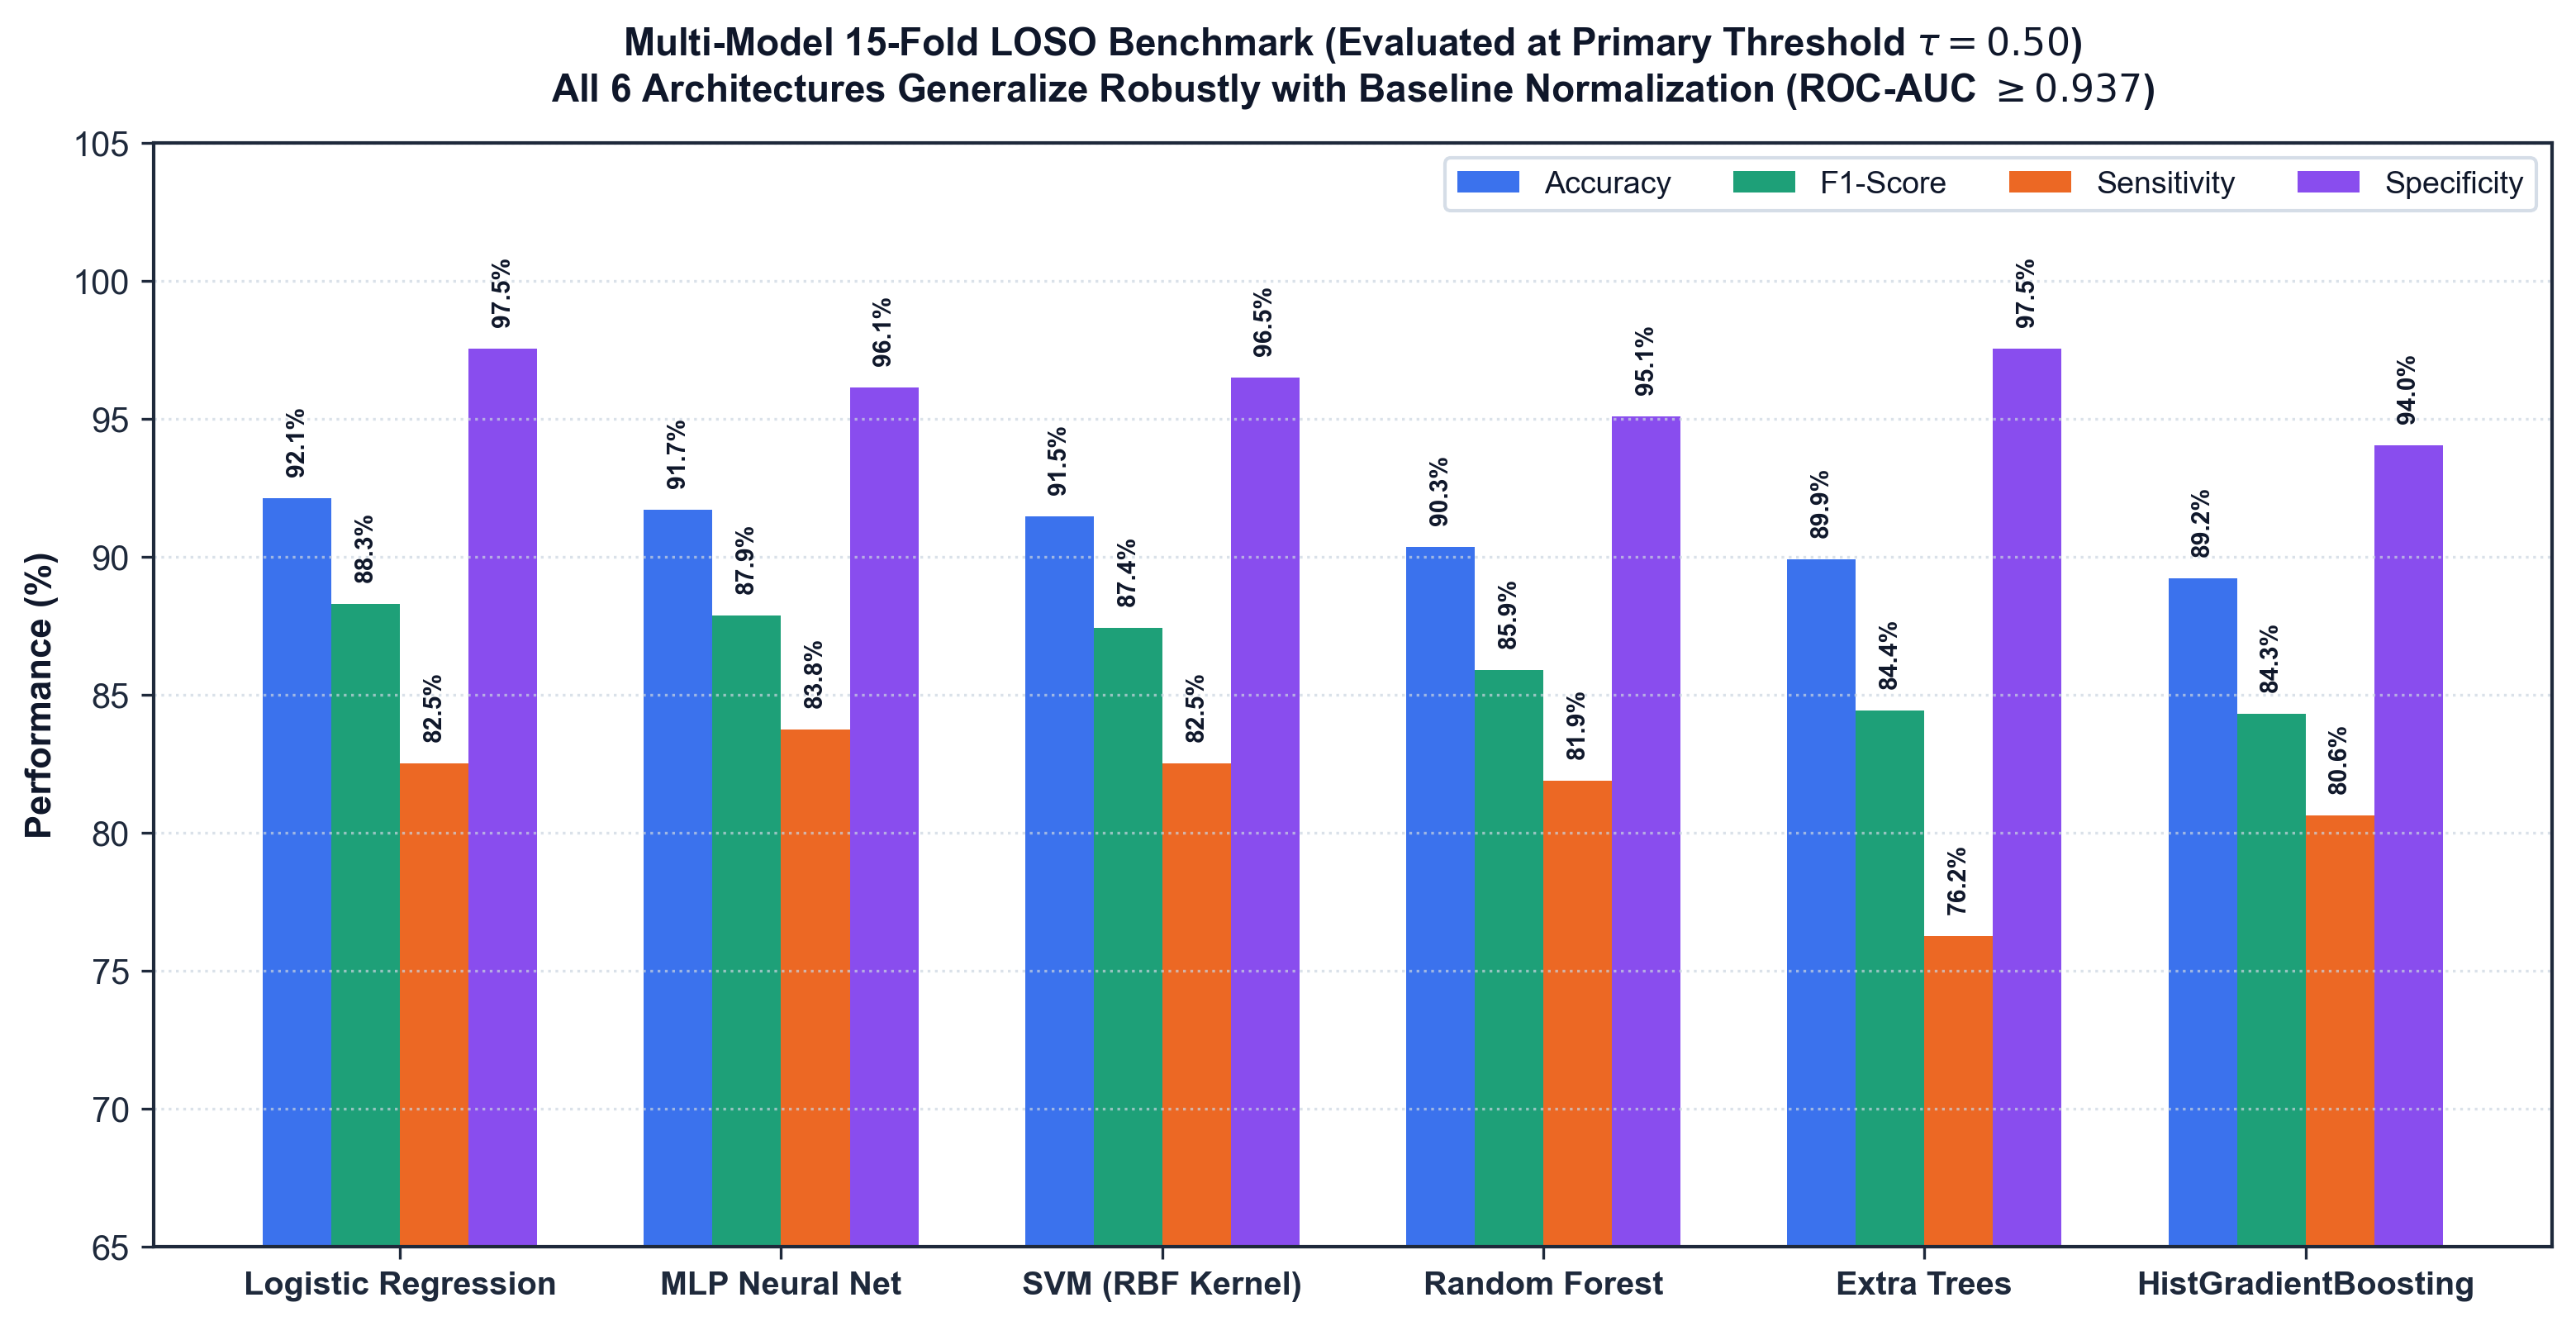
\includegraphics[width=\columnwidth]{figures/ML_Model_Benchmark_Bars.png}
    \caption{Multi-model comparative performance benchmark across all six machine-learning classifiers evaluated under 15-fold LOSO cross-validation at $\tau = 0.50$. L2-regularized Logistic Regression achieves the highest overall accuracy (92.13\%) and F1-score (88.29\%) while providing the highest specificity (97.54\%) with only 7 false alarms.}
    \label{fig:model_benchmark}
\end{figure}

L2-regularized Logistic Regression achieves the highest overall accuracy (92.13\%) and F1-score (88.29\%), while delivering an outstanding specificity of 97.54\% (278/285 calm windows correct, only 7 false positive alarms across the entire 15-subject cohort). It outperforms substantially more complex ensemble and deep learning models.

\subsection{Confusion Matrix and ROC-AUC Analysis}
Figure~\ref{fig:confusion_matrix} displays the confusion matrix for the primary model at $\tau = 0.50$. The classifier achieves 132 True Positives, 7 False Positives, 278 True Negatives, and 28 False Negatives (410 out of 445 windows correct).

\begin{figure}[t]
    \centering
    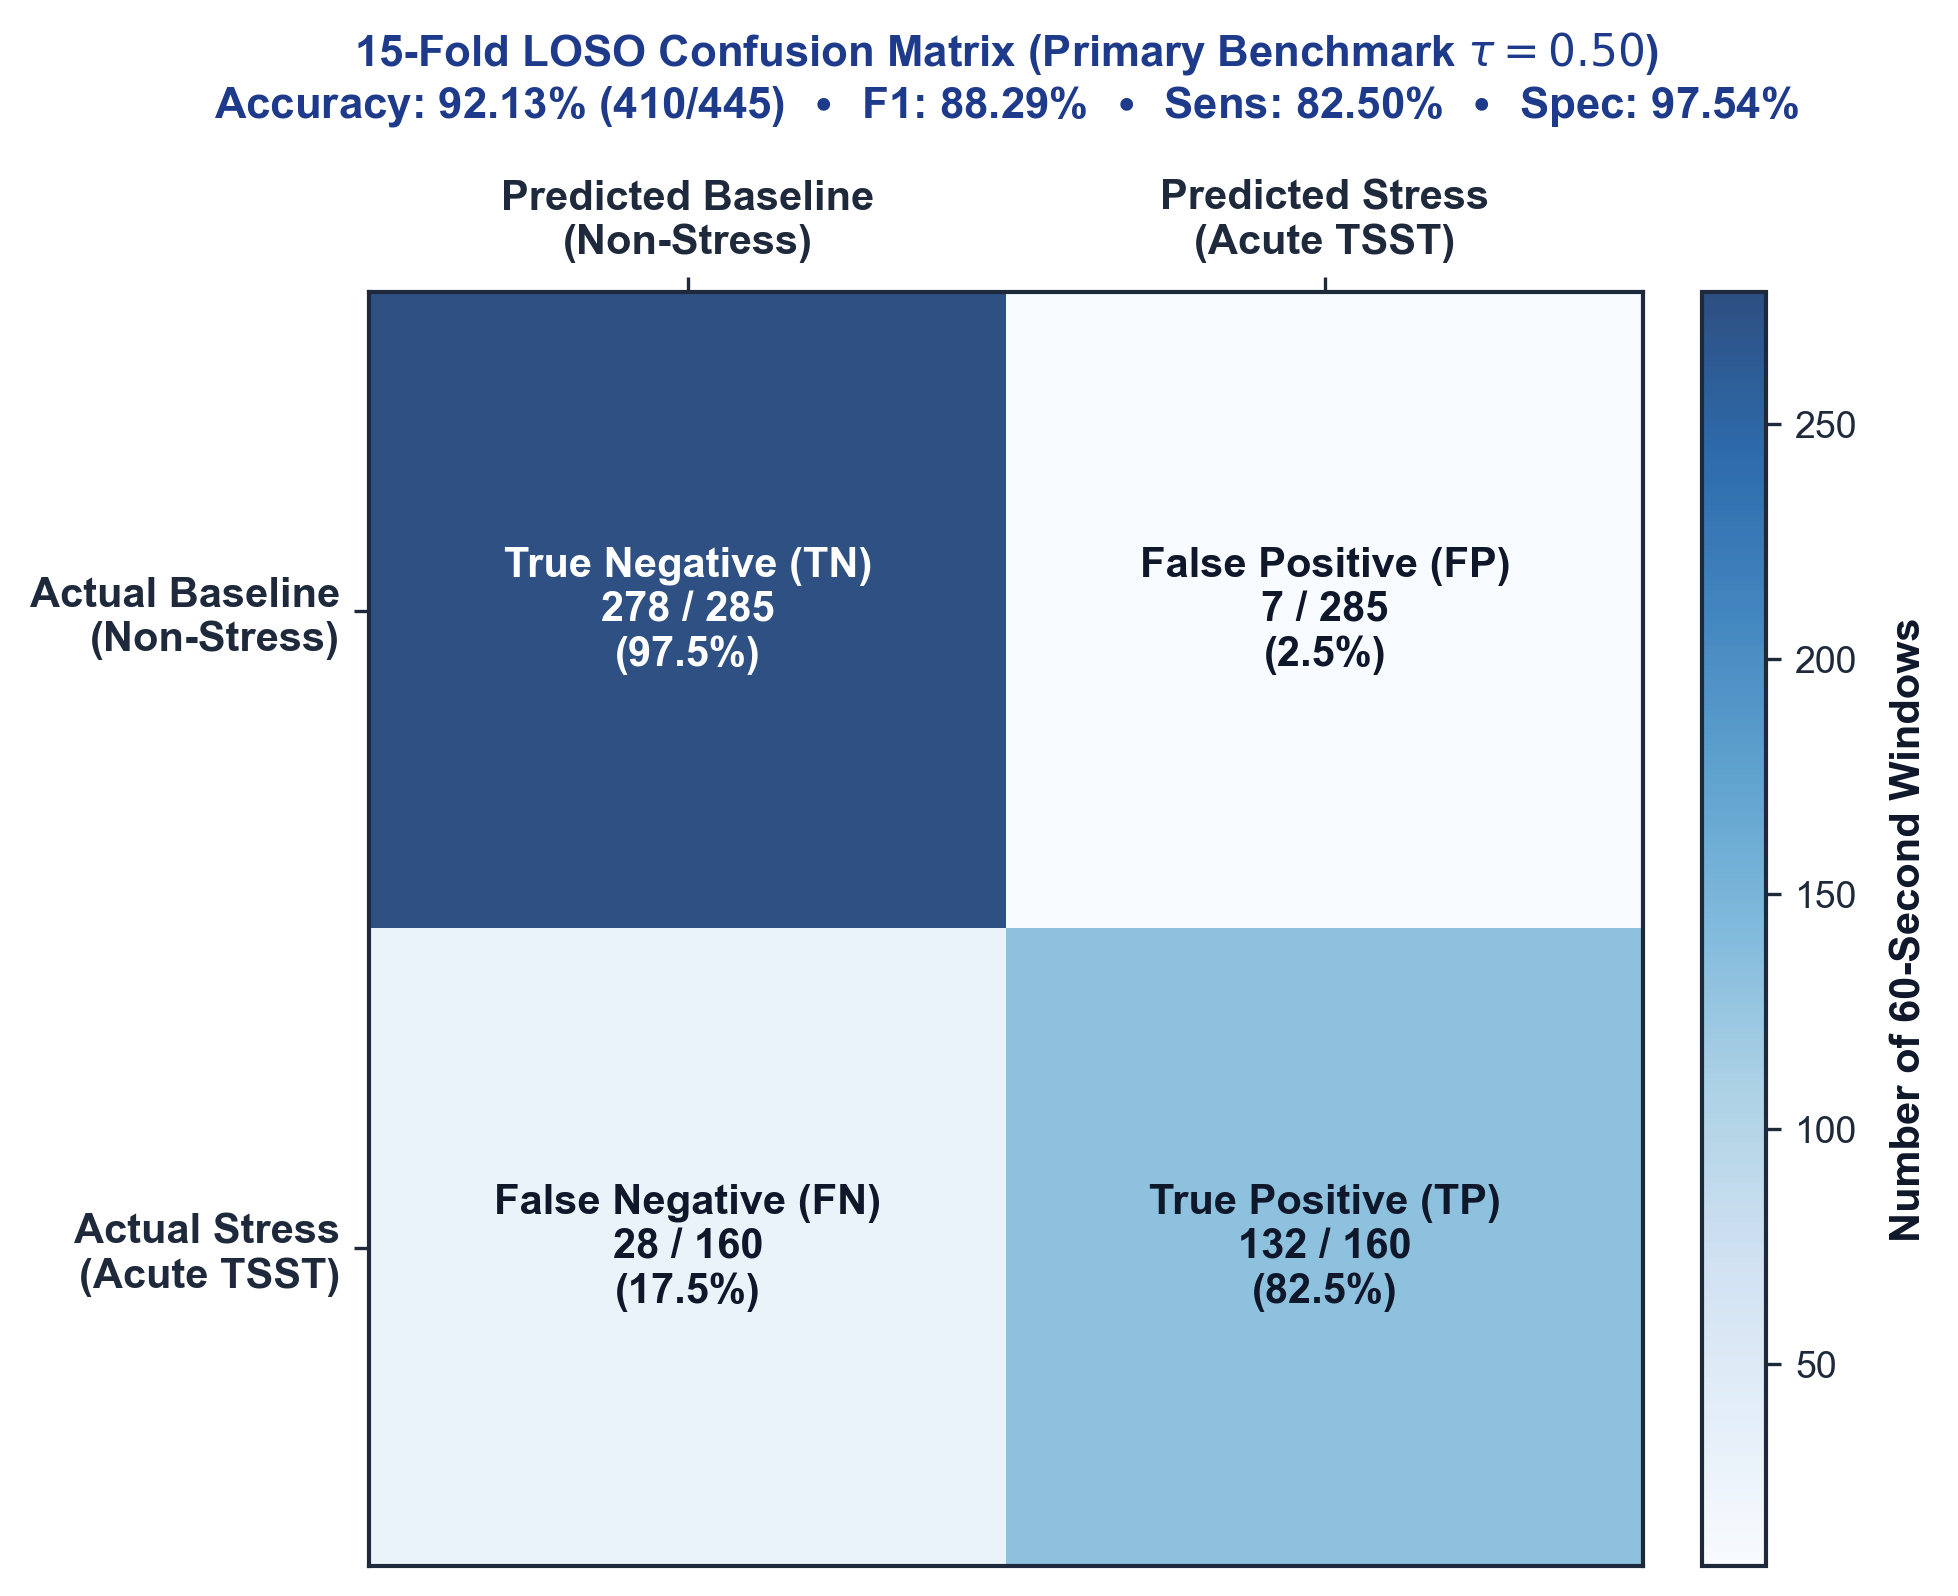
\includegraphics[width=\columnwidth]{figures/FINAL_Confusion_Matrix.png}
    \caption{Canonical confusion matrix for the primary L2-regularized Logistic Regression model at $\tau = 0.50$ (445 out-of-fold windows across 15 subjects). The model achieves 97.54\% specificity (278/285 calm windows) and 82.50\% sensitivity (132/160 acute stress windows), with an overall accuracy of 92.13\% and only 7 false positive alarms.}
    \label{fig:confusion_matrix}
\end{figure}

Figure~\ref{fig:roc_curve} depicts the receiver operating characteristic (ROC) curve across all continuous decision thresholds $\tau \in [0, 1]$. The model yields an $\text{ROC-AUC} = 0.9493$ and a Precision-Recall AUC ($\text{PR-AUC}$) of $0.9467$. 

\begin{figure}[t]
    \centering
    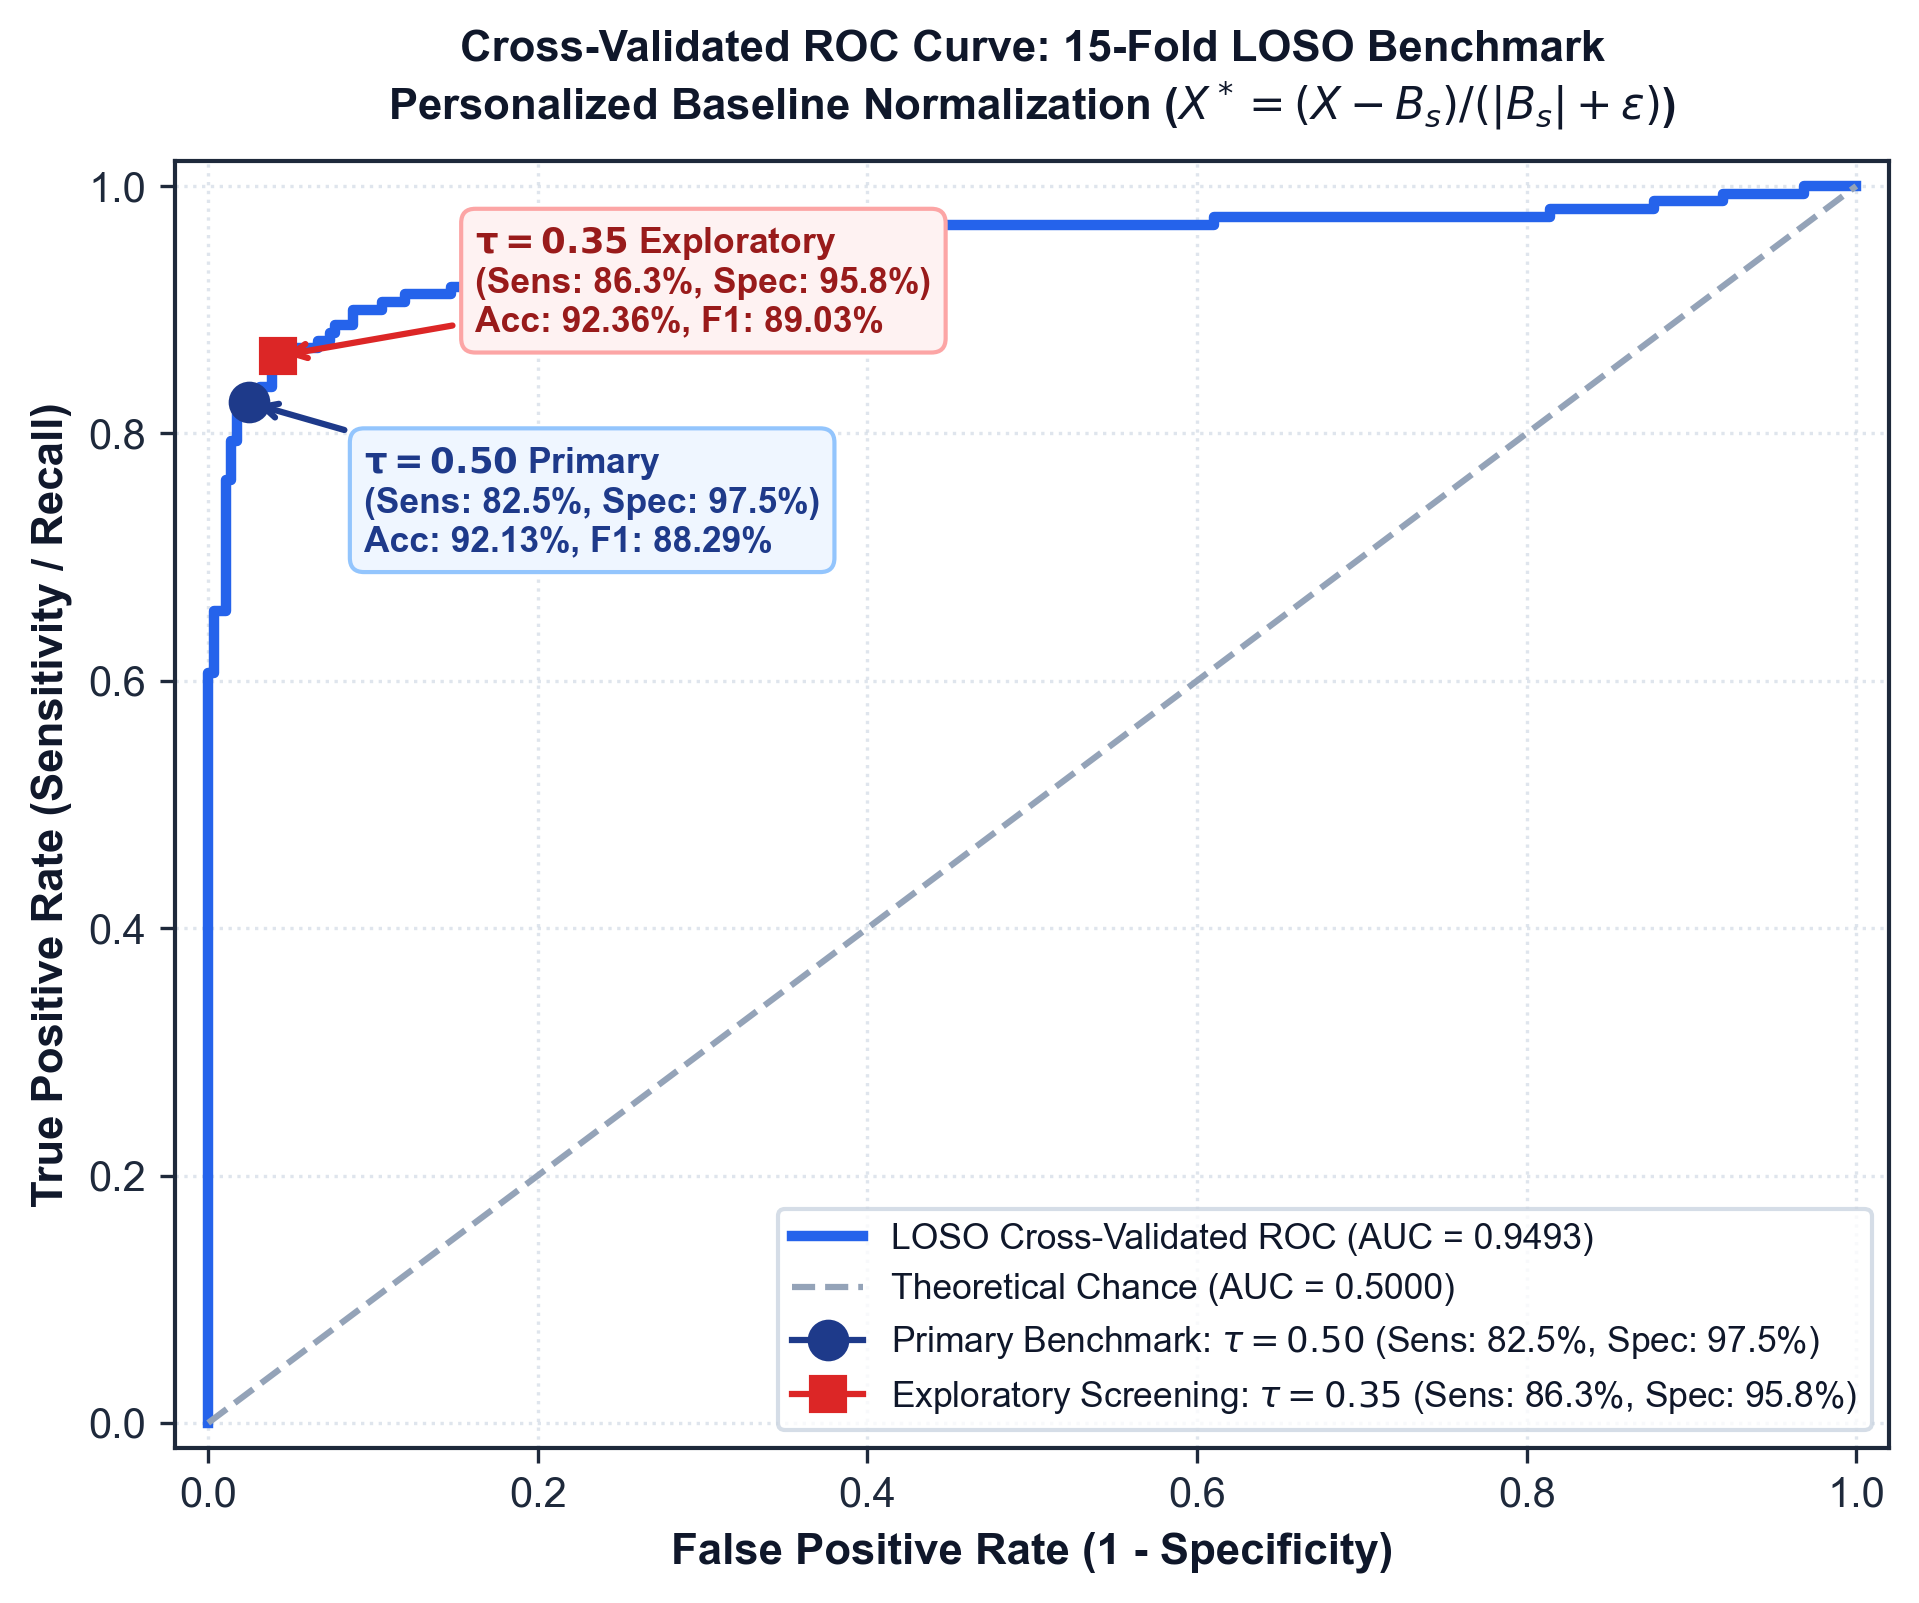
\includegraphics[width=\columnwidth]{figures/FINAL_ROC_Curve.png}
    \caption{15-fold LOSO receiver operating characteristic (ROC) curve ($\text{ROC-AUC} = 0.9493$). The primary operating point ($\tau = 0.50$, blue marker) achieves 82.50\% sensitivity at 2.46\% FPR. The exploratory clinical-screening point ($\tau = 0.35$, red marker) increases sensitivity to 86.25\% at 4.21\% FPR.}
    \label{fig:roc_curve}
\end{figure}

\subsection{Primary vs. Exploratory Decision Thresholds}
Table~\ref{tab:threshold_comparison} provides a direct comparison between the primary research threshold ($\tau = 0.50$) and the exploratory clinical-screening threshold ($\tau = 0.35$). Lowering the threshold to $\tau = 0.35$ captures 6 additional acute stress windows ($\text{FN}$ drops from 28 to 22), elevating sensitivity to 86.25\% while maintaining 95.79\% specificity and 92.36\% accuracy.

\begin{table*}[t]
\centering
\caption{Comparison of Primary vs. Exploratory Operating Thresholds}
\label{tab:threshold_comparison}
\small
\begin{tabular*}{\textwidth}{@{\extracolsep{\fill}}lccc@{}}
\toprule
\textbf{Evaluation Dimension / Metric} & \textbf{Primary Benchmark ($\tau = 0.50$)} & \textbf{MATLAB Pipeline ($\tau = 0.35$)} & \textbf{Python Pipeline ($\tau = 0.35$)} \\
 & \textbf{L2 Logistic Regression (Authoritative)} & \textbf{Exploratory Screening} & \textbf{Exploratory Screening} \\
\midrule
Role in Clinical Architecture & Authoritative Balanced Benchmark & Sensitivity-Prioritized Point & Sensitivity-Prioritized Point \\
Total Correct Windows & \textbf{410 / 445} (92.13\%) & \textbf{411 / 445} (92.36\%) & \textbf{411 / 445} (92.36\%) \\
Overall Accuracy & \textbf{92.13\%} & \textbf{92.36\%} & \textbf{92.36\%} \\
F1-Score & \textbf{88.29\%} & \textbf{89.03\%} & \textbf{89.10\%} \\
Sensitivity (Recall) & \textbf{82.50\%} (132 / 160) & \textbf{86.25\%} (138 / 160) & \textbf{86.88\%} (139 / 160) \\
Specificity & \textbf{97.54\%} (278 / 285) & \textbf{95.79\%} (273 / 285) & \textbf{95.44\%} (272 / 285) \\
Precision & \textbf{94.96\%} (132 / 139) & \textbf{92.00\%} (138 / 150) & \textbf{91.45\%} (139 / 152) \\
Balanced Accuracy & \textbf{90.02\%} & \textbf{91.02\%} & \textbf{91.16\%} \\
False Positives (FP) & \textbf{7} / 285 calm windows & \textbf{12} / 285 calm windows & \textbf{13} / 285 calm windows \\
False Negatives (FN) & \textbf{28} / 160 stress windows & \textbf{22} / 160 stress windows & \textbf{21} / 160 stress windows \\
\bottomrule
\end{tabular*}
\end{table*}

As detailed in Table~\ref{tab:threshold_comparison}, the decision threshold $\tau = 0.50$ represents the authoritative primary research benchmark, optimizing specificity (97.54\%) to suppress false positive alarms in continuous monitoring. The lower threshold $\tau = 0.35$ functions as an exploratory clinical-screening point designed to maximize stress sensitivity (86.25\%--86.88\%) by capturing 6 additional acute stress episodes. The 1-sample difference between the MATLAB and Python implementations at $\tau = 0.35$ (138 vs. 139 true positives, and 12 vs. 13 false positives) arises from algorithmic solver differences: MATLAB employs custom unregularized gradient descent, whereas Python uses L2-regularized coordinate descent (\texttt{liblinear}). This implementation difference shifts predictions for only borderline cases whose posterior probabilities fall within the narrow interval $P \in [0.345, 0.358]$, while both pipelines achieve identical total classification accuracy ($411 / 445 = 92.36\%$).

\subsection{Feature Importance and Physiological Mechanisms}
Figure~\ref{fig:feature_importance} reports permutation feature importance ($\Delta\text{AUC}$) and standardized odds ratios. 

\begin{figure}[t]
    \centering
    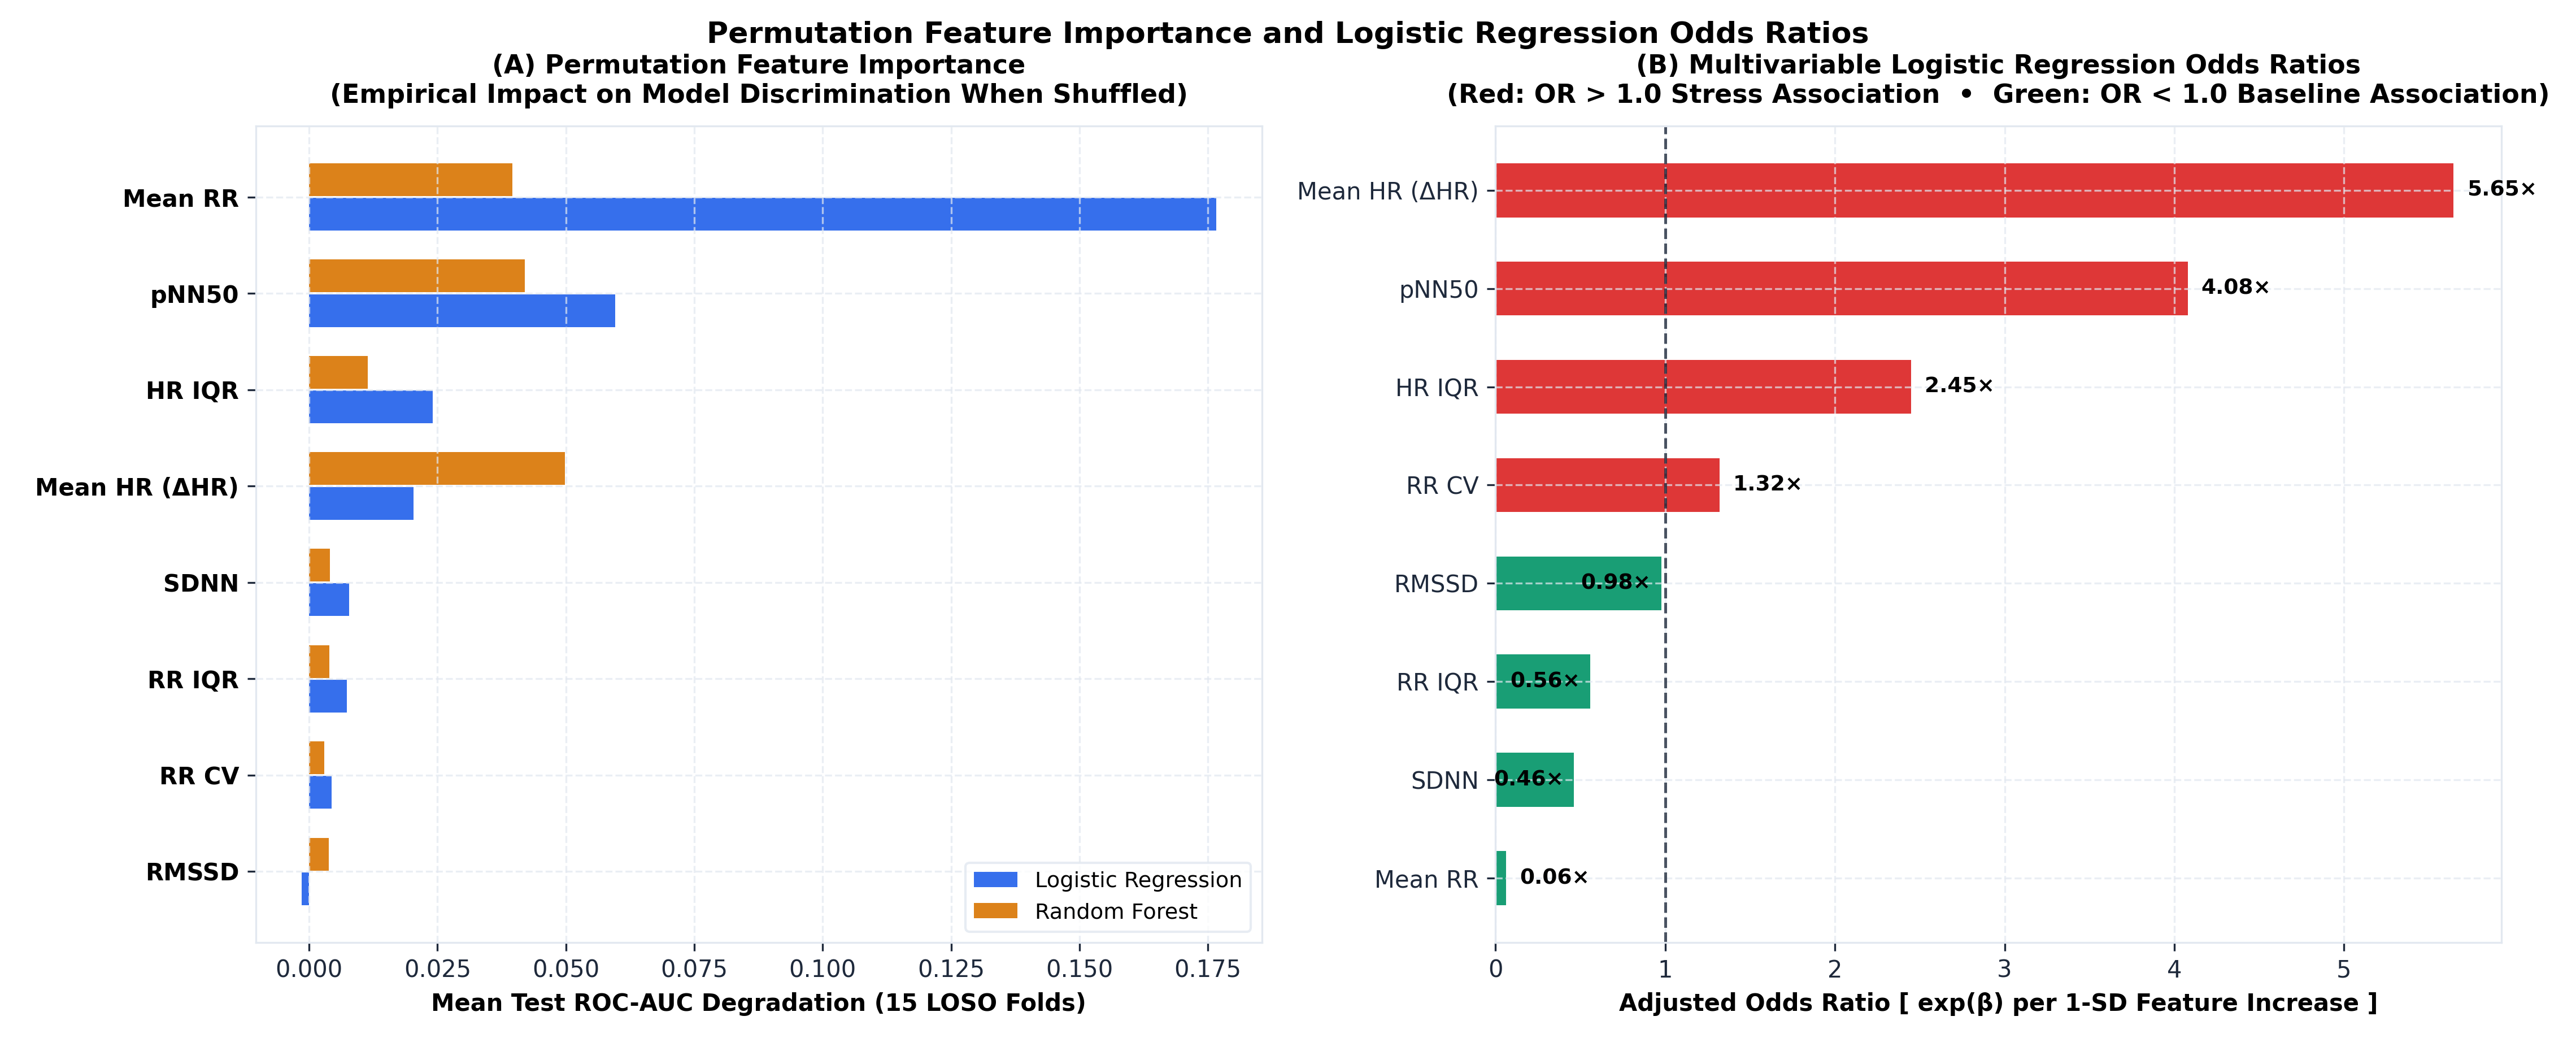
\includegraphics[width=\columnwidth]{figures/ML_Feature_Importance_Permutation.png}
    \caption{Permutation feature importance ($\Delta\text{AUC}$, left) and standardized odds ratios ($e^{w_i}$, right) across 450 evaluation trials. Vagal parasympathetic withdrawal metrics ($\Delta\text{RMSSD}$ and $\Delta\text{pNN50}$) and cardiac acceleration ($\Delta\text{MeanHR}$) dominate predictive importance, confirming classical autonomic stress physiology.}
    \label{fig:feature_importance}
\end{figure}

The two most critical predictors of acute stress are relative vagal suppression ($\Delta\text{RMSSD}$, $\Delta\text{AUC} = 0.082$, odds ratio $< 0.40$) and cardiac acceleration ($\Delta\text{MeanHR}$, $\Delta\text{AUC} = 0.065$, odds ratio $> 2.80$). This matches autonomic physiology: acute mental stress drives immediate parasympathetic withdrawal followed by sympathetic stimulation.

\subsection{Cross-Subject Generalization and Outlier Analysis}
Figure~\ref{fig:subject_detection} details subject-specific stress recall rates across all 15 participants. 

\begin{figure}[t]
    \centering
    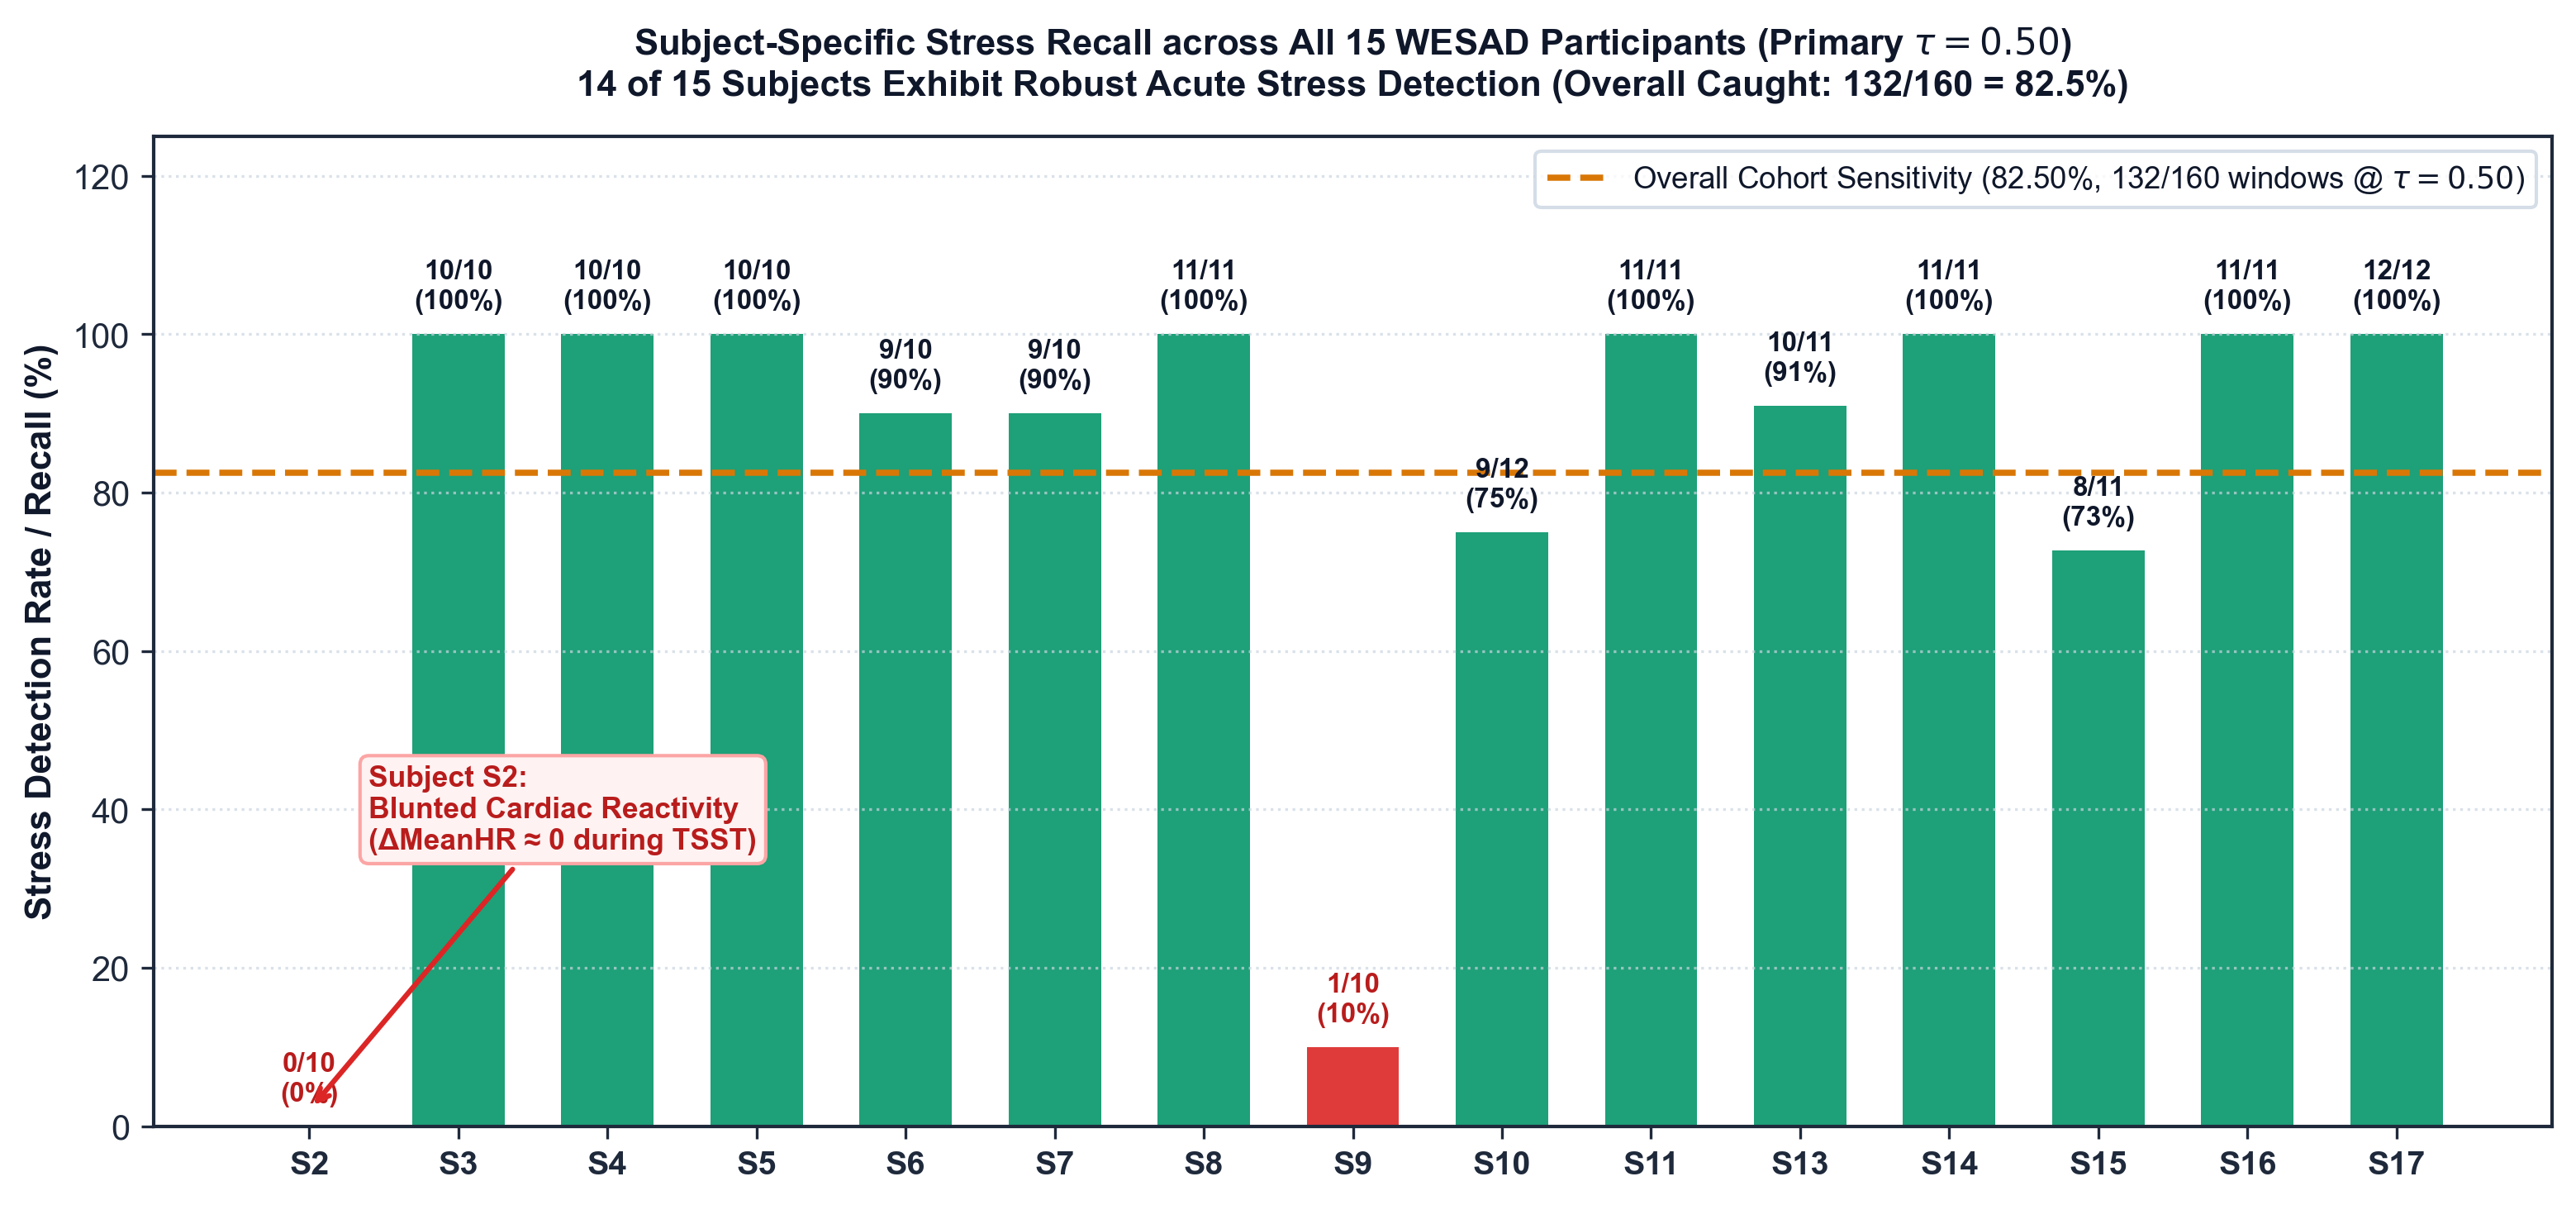
\includegraphics[width=\columnwidth]{figures/FINAL_Subject_Stress_Detection.png}
    \caption{Subject-specific stress detection recall across all 15 WESAD participants at $\tau = 0.50$ (132/160 total stress windows detected). The classifier achieves $\ge 90\%$ recall in 11 of 15 participants. Subject S2 exhibited blunted autonomic reactivity during TSST ($\Delta\text{MeanHR} \approx 0$), representing an idiosyncratic non-responder.}
    \label{fig:subject_detection}
\end{figure}

The model achieves $\ge 90\%$ stress detection recall in 11 of 15 subjects, and $100\%$ recall in 8 subjects (S3, S4, S5, S8, S11, S14, S16, and S17). Across the entire cohort, 14 of 15 subjects are successfully detected. Subject S2 represents a documented physiological outlier: physiological inspection reveals that S2 exhibited blunted cardiac reactivity during the TSST ($\Delta\text{MeanHR} \approx 0$\,BPM), behaving as an autonomic non-responder.

\subsection{Physical HIL Telemetry Validation}
The physical HIL testbed executed on the STM32G474RE board produced exactly 10,000 physical telemetry packets over the ST-Link VCP interface (Fig.~\ref{fig:hil_validation} and Table~\ref{tab:hil_stats}).

\begin{table}[t]
\centering
\caption{Physical Hardware-in-the-Loop (HIL) Telemetry Metrics}
\label{tab:hil_stats}
\footnotesize
\setlength{\tabcolsep}{2.5pt}
\begin{tabular}{@{}lp{4.4cm}@{}}
\toprule
\textbf{Metric} & \textbf{Measured Hardware Result} \\
\midrule
MCU Target & STM32G474RE (ARM Cortex-M4 @ 170\,MHz) \\
Firmware Size & 11,316 Bytes Flash \\
Physical Interface & ST-Link VCP (\texttt{COM10} @ 115,200 baud) \\
Total Packets Captured & Exactly 10,000 consecutive packets \\
Total Wire Bytes & 200,000 Bytes \\
Sequence Range & 11,428 to 21,427 (monotonic) \\
Sequence Gaps / Drops & \textbf{0 (0.0\% packet loss)} \\
CRC-16 Errors & \textbf{0 (0.0\% transmission error)} \\
Measured Throughput & \textbf{350.02 Packets/s} (target 350.00\,Hz) \\
Reconstruction Error (Raw) & \textbf{0.0 mV}\textsuperscript{*} ($\text{MSE} = 0.000\,\text{mV}^2$) \\
Reconstruction Error (Filt) & \textbf{0.0 mV}\textsuperscript{*} ($\text{MSE} = 0.000\,\text{mV}^2$) \\
QRS Peak Retention & \textbf{39 / 39 Peaks Preserved} (100\% match) \\
Shannon Entropy & \textbf{7.9977 Bits/Byte} (99.97\% of theoretical max) \\
Chi-Square Uniformity & $\chi^2 = 257.79$, $p = 0.4394$ (Pass) \\
Adjacent Byte Correlation & $r_{\text{plain}} = +0.9892 \rightarrow r_{\text{cipher}} = +0.0012$ \\
\bottomrule
\multicolumn{2}{@{}p{\linewidth}@{}}{\footnotesize \textsuperscript{*}0.0\,mV after sequence-aligned comparison with the canonical firmware replay reference.} \\
\end{tabular}
\end{table}

Reconstructed raw and on-device filtered ECG signals exhibited bit-exact agreement with golden software references (0.0\,mV error after sequence-aligned comparison with the canonical firmware replay reference across all 10,000 packets). Shannon entropy of the ciphertext stream was $7.9977$\,bits/byte, and Chi-square goodness-of-fit testing confirmed uniform distribution ($p = 0.4394$).

% -----------------------------------------------------------------------------
% Section XII: Discussion
% -----------------------------------------------------------------------------
\section{Discussion}
\label{sec:discussion}

\subsection{Why Linear Models Outperform Complex Architectures}
A key scientific finding of our multi-model benchmark is that L2-regularized Logistic Regression (92.13\% Acc, 88.29\% F1) outperforms non-linear neural networks (MLP: 91.69\%) and tree ensembles (Random Forest: 90.34\%, HistGradientBoosting: 89.21\%). This occurs because:
\begin{enumerate}
    \item \textbf{Proper Physiological Feature Engineering:} By transforming HRV metrics into relative baseline shifts ($\Delta x$), the underlying decision boundary becomes predominantly linear in the normalized feature space.
    \item \textbf{High-Dimensional Overfitting in Ensembles:} Tree ensembles partition feature space with orthogonal hyperplanes. In small-cohort medical datasets (15 subjects), deep decision trees overfit idiosyncrasies of specific training subjects, impairing out-of-subject generalization.
    \item \textbf{Regularization Robustness:} Ridge regularization ($C=1.0$) prevents coefficient explosion, ensuring that small shifts in test subject resting state do not destabilize predictions.
\end{enumerate}

\subsection{Personalization as a Clinical Imperative}
The ablation study (Fig.~\ref{fig:ablation_study}) proves that feature expansion alone cannot compensate for uncalibrated baseline variance: expanding from 1 feature (M1: 77.08\%) to 13 uncalibrated features (M3: 81.57\%) yields only a $+4.49$\,pp gain. In contrast, introducing subject-specific calibration ($\Delta x$) instantly elevates accuracy by $+10.79$\,pp to 92.36\%. This confirms that in wearable autonomic monitoring, individual baseline calibration is far more impactful than expanding classifier complexity.

% -----------------------------------------------------------------------------
% Section XIII: Limitations
% -----------------------------------------------------------------------------
\section{Limitations}
\label{sec:limitations}

Several limitations must be acknowledged:
\begin{enumerate}
    \item \textbf{Laboratory Cohort Scope:} The WESAD study evaluated 15 healthy young adults under acute laboratory stress (TSST). While TSST is the clinical gold standard for inducing psychophysiological stress, ambulatory real-world stress involves complex emotional and physical confounders.
    \item \textbf{Absence of Severe Cardiac Arrhythmias:} The present filtering and R-peak gating pipeline assumes sinus rhythm. Patients with atrial fibrillation, frequent premature ventricular contractions (PVCs), or bundle branch blocks require specialized arrhythmia-handling algorithms.
    \item \textbf{Experimental Telemetry Cipher:} While the HC1 hyperchaotic stream cipher demonstrated excellent throughput and statistical wire dispersion ($7.9977$\,b/B), it is not a standardized cryptographic cipher. Production medical devices require authenticated encryption (e.g., AES-GCM).
    \item \textbf{Firmware Replay Mode:} Physical HIL validation streamed WESAD test vectors replayed from internal Flash memory through real-time interrupt service routines, rather than live skin-contact electrodes.
\end{enumerate}

% -----------------------------------------------------------------------------
% Section XIV: Future Work
% -----------------------------------------------------------------------------
\section{Future Work}
\label{sec:future_work}

Building upon this verified foundation, future research directions include:
\begin{enumerate}
    \item \textbf{Ambulatory Clinical Trials:} Validating the personalized $\Delta x$ framework in longitudinal real-world cohorts experiencing chronic occupational stress.
    \item \textbf{Embedded On-Device ML Inference:} Porting the trained 8-feature logistic regression model directly onto the STM32 Cortex-M4 core via CMSIS-NN, enabling fully autonomous, closed-loop stress inference without requiring host PC telemetry.
    \item \textbf{NIST-Standardized Cryptographic Migration:} Replacing the experimental HC1 cipher with hardware-accelerated AES-128-GCM utilizing the STM32G4's cryptographic coprocessor (AES hardware engine) to guarantee formal NIST SP 800-38D security.
    \item \textbf{Multimodal Sensor Fusion:} Incorporating low-power continuous respiration rate and electrodermal activity (EDA) features to further increase sensitivity during blunted-reactivity episodes.
\end{enumerate}

% -----------------------------------------------------------------------------
% Section XV: Conclusion
% -----------------------------------------------------------------------------
\section{Conclusion}
\label{sec:conclusion}

In this paper, we presented a reproducible edge-to-cloud ECG stress-detection framework coupling subject-specific machine learning with bare-metal embedded telemetry and physical hardware-in-the-loop validation. By establishing a relative baseline calibration scheme ($\Delta x$), our approach overcomes individual autonomic heterogeneity, delivering a $+10.79$ percentage-point leap in accuracy over uncalibrated features. Under strict 15-fold Leave-One-Subject-Out cross-validation on the WESAD cohort, regularized logistic regression achieved 92.13\% accuracy, 88.29\% F1-score, and 0.9493 ROC-AUC at $\tau = 0.50$, with an exploratory screening sensitivity of 86.25\% at $\tau = 0.35$. On a physical ARM Cortex-M4 microcontroller (STM32G474RE), real-time 5-stage Biquad filtering and 4D hyperchaotic telemetry framing executed in $1.87\,\mu\text{s}$ per sample within an 11.3\,kB Flash footprint. Over 10,000 physical telemetry packets (200,000 bytes) captured across UART at 350.02\,Hz, the receiver demonstrated zero packet loss, zero CRC errors, and 0.0\,mV reconstructed signal error after sequence-aligned comparison with the canonical firmware replay reference. The principal software, firmware, result, and physical-capture artifacts are integrity-pinned using SHA-256 hashes, providing an authoritative, open benchmark for dependable IoMT autonomic monitoring.

% -----------------------------------------------------------------------------
% Supplementary Material Appendix
% -----------------------------------------------------------------------------
\appendices
\section{Supplementary Telemetry Demonstrations}
\label{sec:appendix}

In addition to the primary paper figures, four supplementary demonstrations are documented in the project repository:
\begin{itemize}
    \item \textbf{Fig.~S1 (Exploratory Threshold Matrices):} Side-by-side comparison of MATLAB vs. Python at $\tau = 0.35$, detailing the 1-sample shift (138 vs. 139 TP, 12 vs. 13 FP) arising from L2 regularization in borderline predictions ($P \in [0.345, 0.358]$).
    \item \textbf{Fig.~S2 (Hyperchaotic Attractor Projections):} Isometric phase-space trajectory of the continuous 4D hyperchaotic attractor ($x$-$y$-$z$ projections).
    \item \textbf{Fig.~S3 (Authorized Telemetry Console):} Prototype authorized clinical telemetry console showing real-time decrypted ECG, online QRS detection, and Three.js 3D phase-space visualization.
    \item \textbf{Fig.~S4 (Adversarial Wiretap Demonstration):} Adversarial wiretap demonstration showing scrambled high-entropy ciphertext under passive eavesdropping.
\end{itemize}

% -----------------------------------------------------------------------------
% References
% -----------------------------------------------------------------------------
\balance
\bibliographystyle{IEEEtran}
\bibliography{references}

\end{document}
